\chapter{Smith Waterman}
\section{The scoring model. The BLOSUM62 matrix}
When two sequences are compared the question that needs an answer is:\\How much they are similar?\\
 The scoring model that we want to consider is based on the use of\textit{ Substitutional matrix} and \textit{Gap penalty} in the chosen alignment algorithm.\\Substitutional matrix and Gap penalty have been created to evaluate different mutation processes that can occur (as we can see in Fig. \ref{sw1} ).\\ 
 With a Substitutional matrix we consider amino acids \textit{matching} and \textit{substitutions}. While with the Gap penalty we consider amino acid \textit{insertions} or \textit{deletions}.
               \begin{figure}[h!]
               	\centering
               	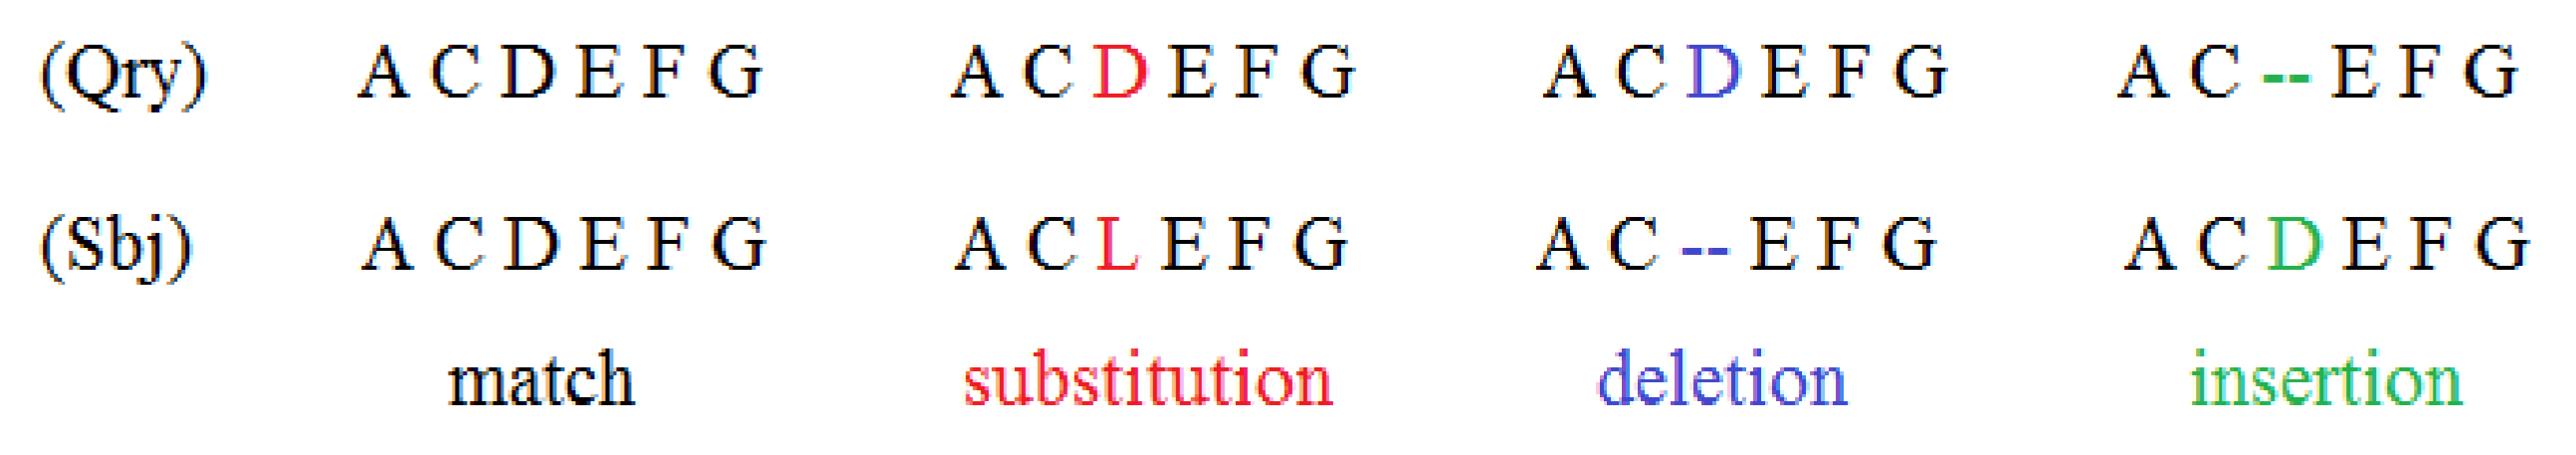
\includegraphics[width=0.85\textwidth]{imm/sw/sw1.png} 	\caption{Alignments with matching, substitution, insertion and deletion.
               		} 
               	\label{sw1}
               \end{figure}
 
 
 
 The BLOSUM62 matrix was introduced in 1992 by Henikoff \& Henikoff \cite{sw-blosum} to give a score for substitution in the amino acid sequence comparisons.
  matrix assigns to each pair of AAs (amino acids), a value that indicates the degree of similarity.
 A positive value in the matrix (Fig. \ref{blosum62}) means that the two amino acids are similar and they are frequently exchanged each other. 
\begin{figure}[h!]
     	\centering
     	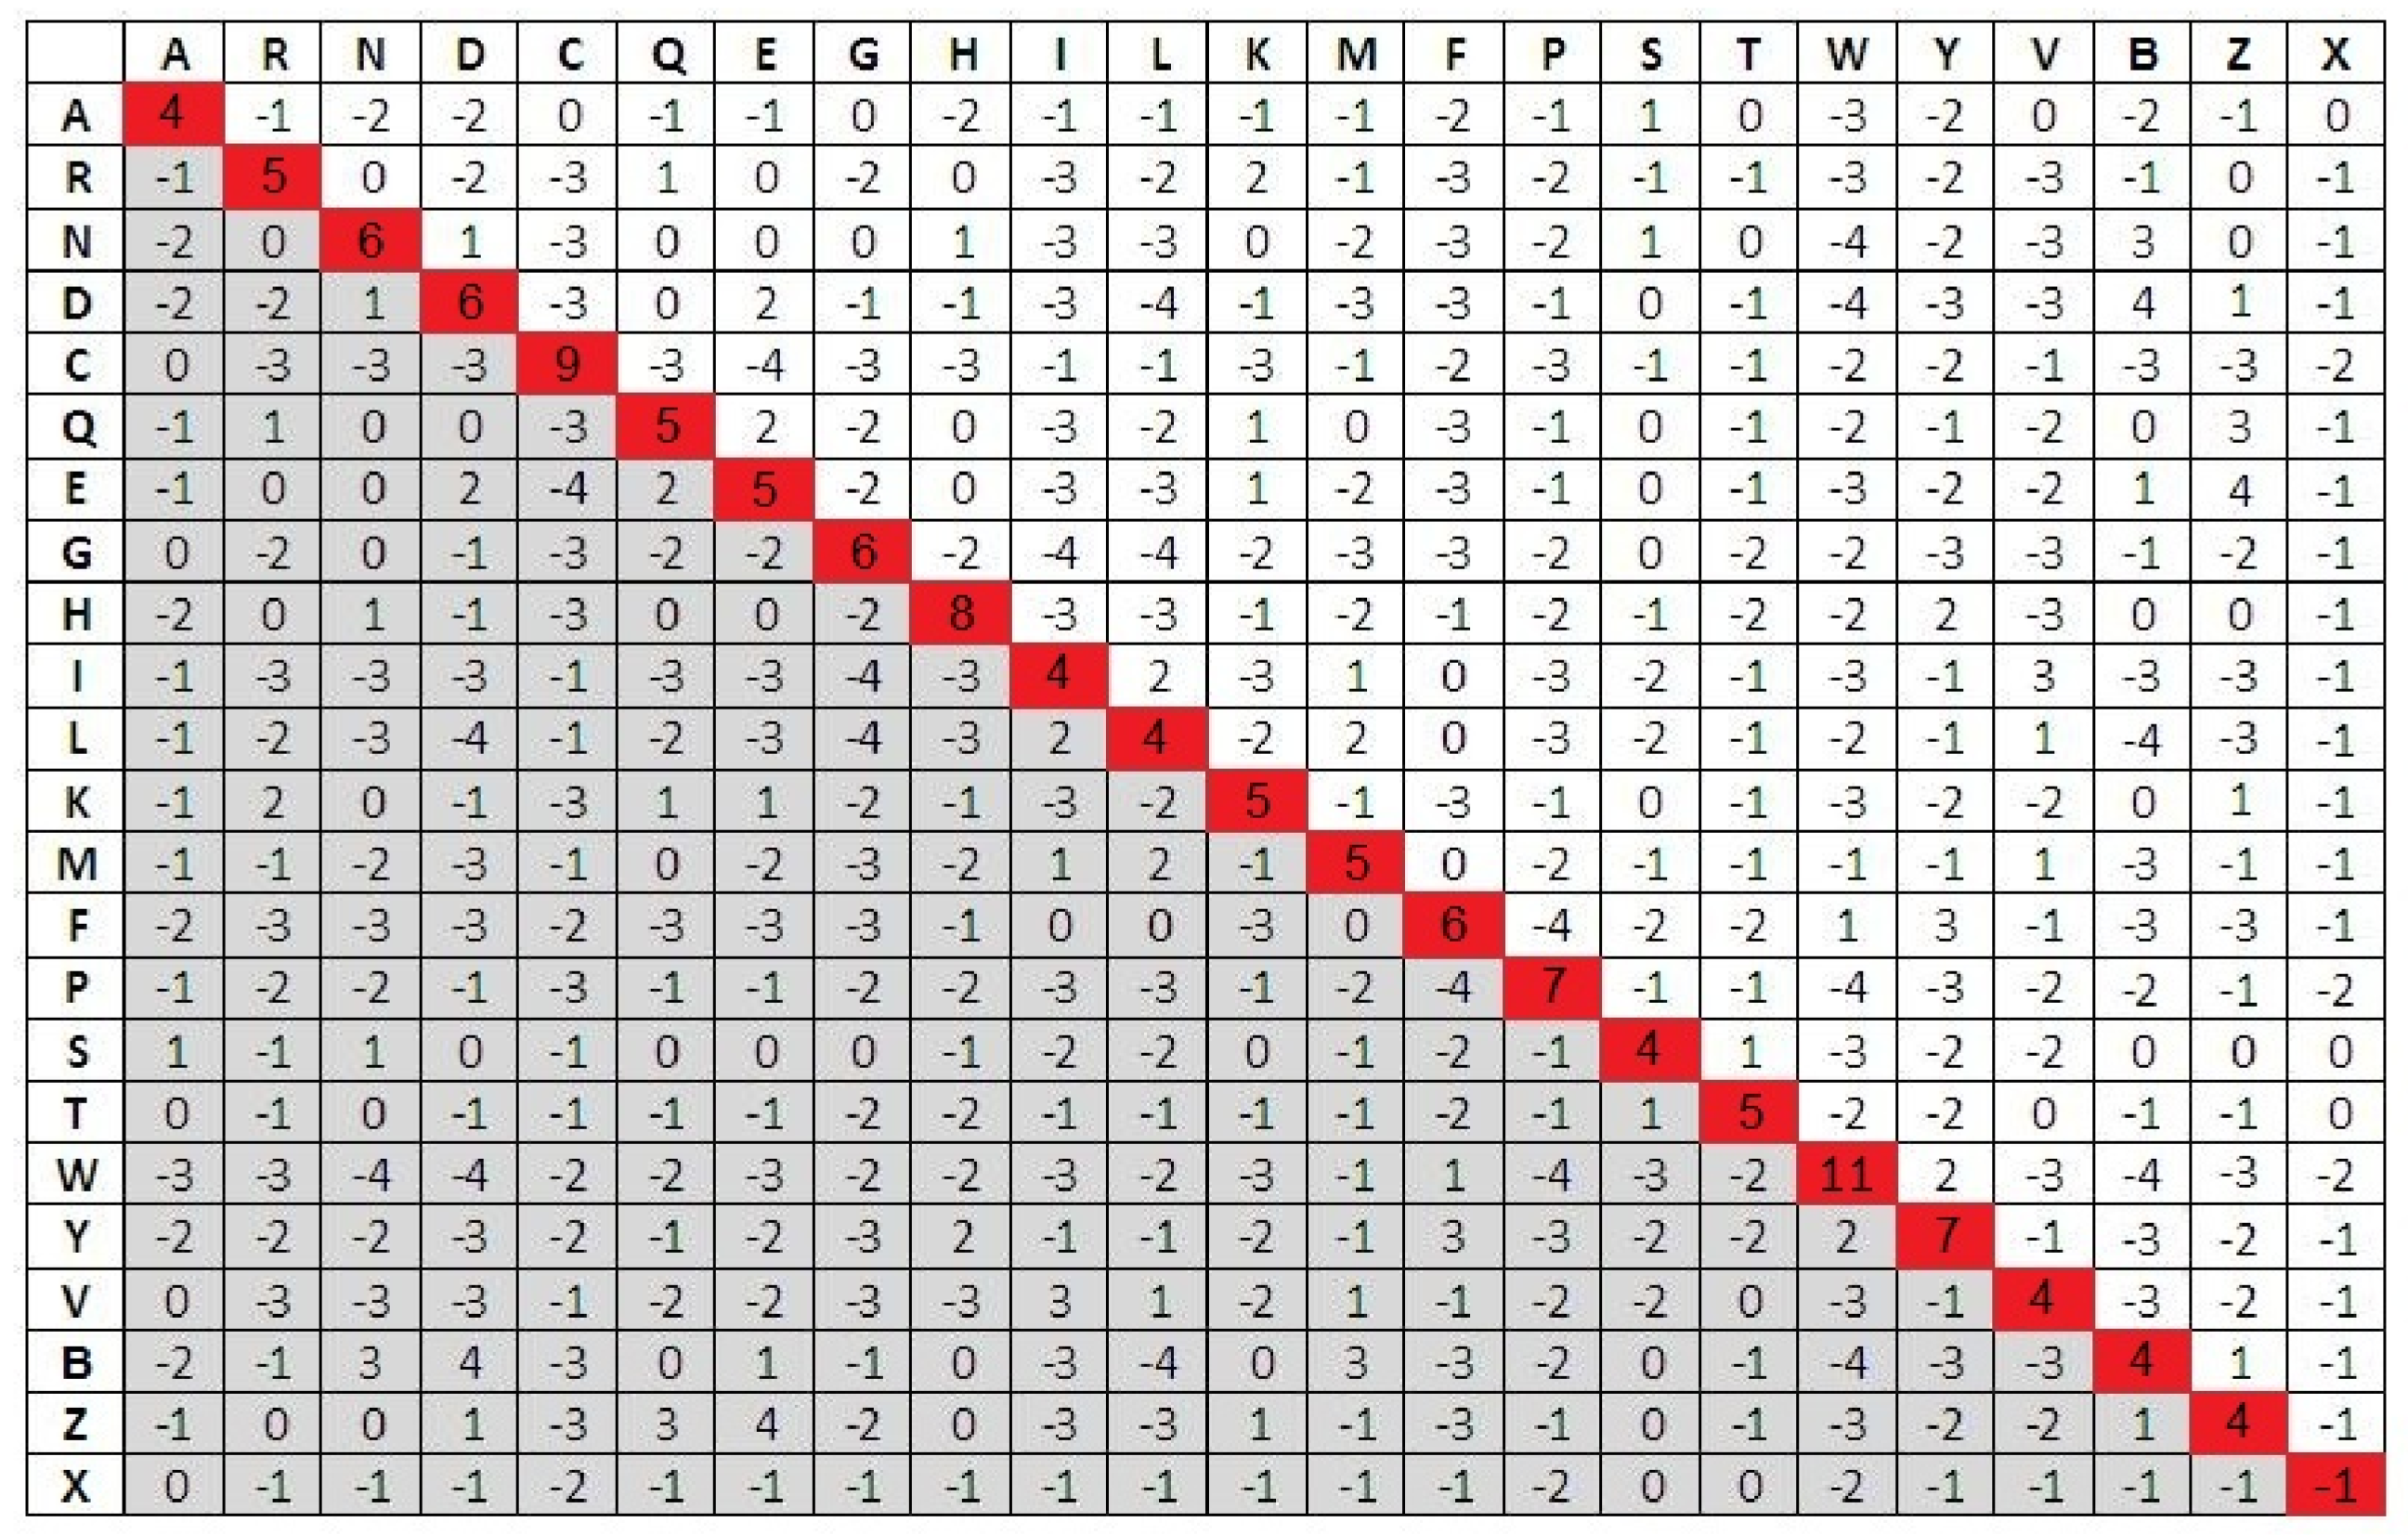
\includegraphics[width=0.85\textwidth]{imm/sw/blosum62.png} 	\caption{The BLOSUM62 substitution matrix.} 
     	\label{blosum62}
\end{figure}
\clearpage
\section{Smith-Waterman Local alignment method	}
Smith and Waterman in 1981 described a Local alignment method whose aim  is to find common regions between two protein (Qry, Sbj) through calculation of similarity score. \\
This algorithm can be substantially described in three steps:
\begin{enumerate}
	\item  \textbf{Initialization}; first row F(i,0) and first column F(0,j) are initialized to 0. Since it is always better to start a new local alignment instead of extend alignments that have got a negative score.
	 \item \textbf{Score matrix filling}; the score is calculated with the Eq. (\ref{sw_eq}) cell by cell.\\
	 \begin{equation}\label{sw_eq}
	 F(i,j) = max \begin{cases}
	
	 0 & \\
	  F(i-1,j-1) + s(Qry(i),Sbj(j))\qquad &\\
	   F(i-1,j)-d &\\
	   F(i,j-1)-d &
	 \end{cases} 
	 \end{equation}
	  if the first term '0' in the equation is selected as max it means that the previous alignment is ended or not alignment is possible. \\Since this algorithm evaluates local alignments, in this matrix there are not negative score.
	 \item   \textbf{output\_writing}: works concurrently with the second process. It checks, in each clock cycle, if the stored Sbj id is changed. If the Sbj id is different, this process will write on the output file the n of Sbj id and the associated Maximum Alignment Score.
	 
	
\end{enumerate}

\section{Simulation and Test} \label{simtest}
The testbench of this architecture is divided in 3 phases:
\begin{enumerate}
	\item \textbf{sub\_matr\_and\_gap\_load }:  configure the systolic array trough the loading of all the storage registers with values coming from the substitutional matrix and gap files.\\
	\item  \textbf{s\_w\_computation}: It starts when the configuration process is terminated and reads from the DB file the Sbj\_id number and the associated amino acids sequence. In this phase we compute the S-W algorithm. This process is ended when all the database is scanned.\\
	\item \textbf{output\_writing}: It checks, in each clock cycle, if the stored Sbj id is changed. If the Sbj id is different, this process will write on the output file the n. of Sbj id and the associated Maximum Alignment Score.
	
	
	
\end{enumerate}
\begin{figure}[h!]
	\centering
	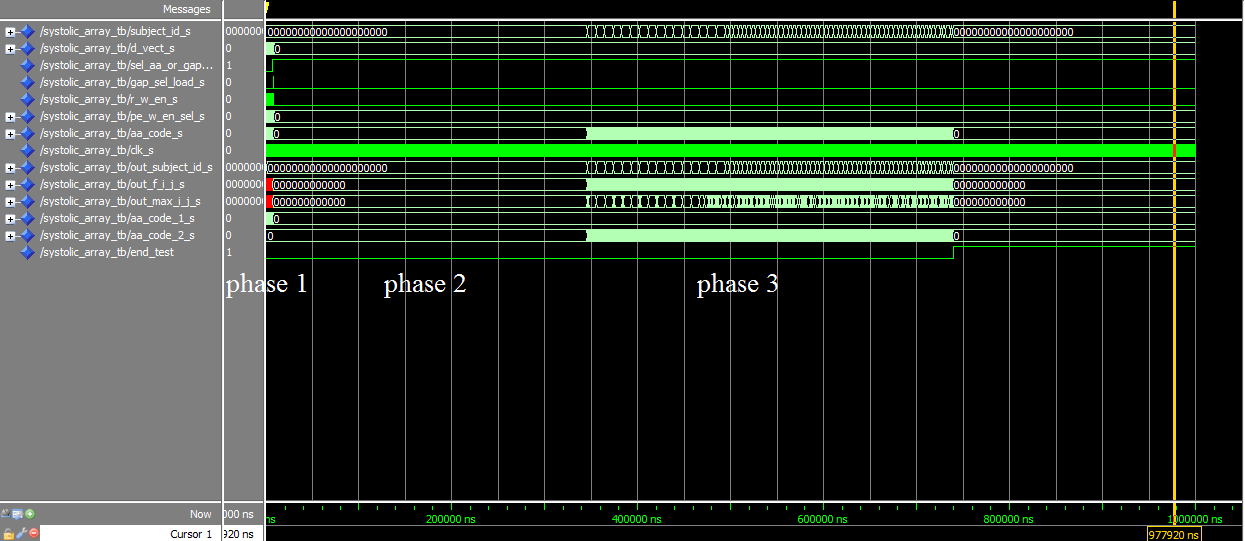
\includegraphics[width=\textwidth]{imm/sw/tb_systolic_array_phases.png} 	\caption{Phases of the testbench} 
	\label{tb_sw}
\end{figure}

\begin{figure}[h!]
	\centering
	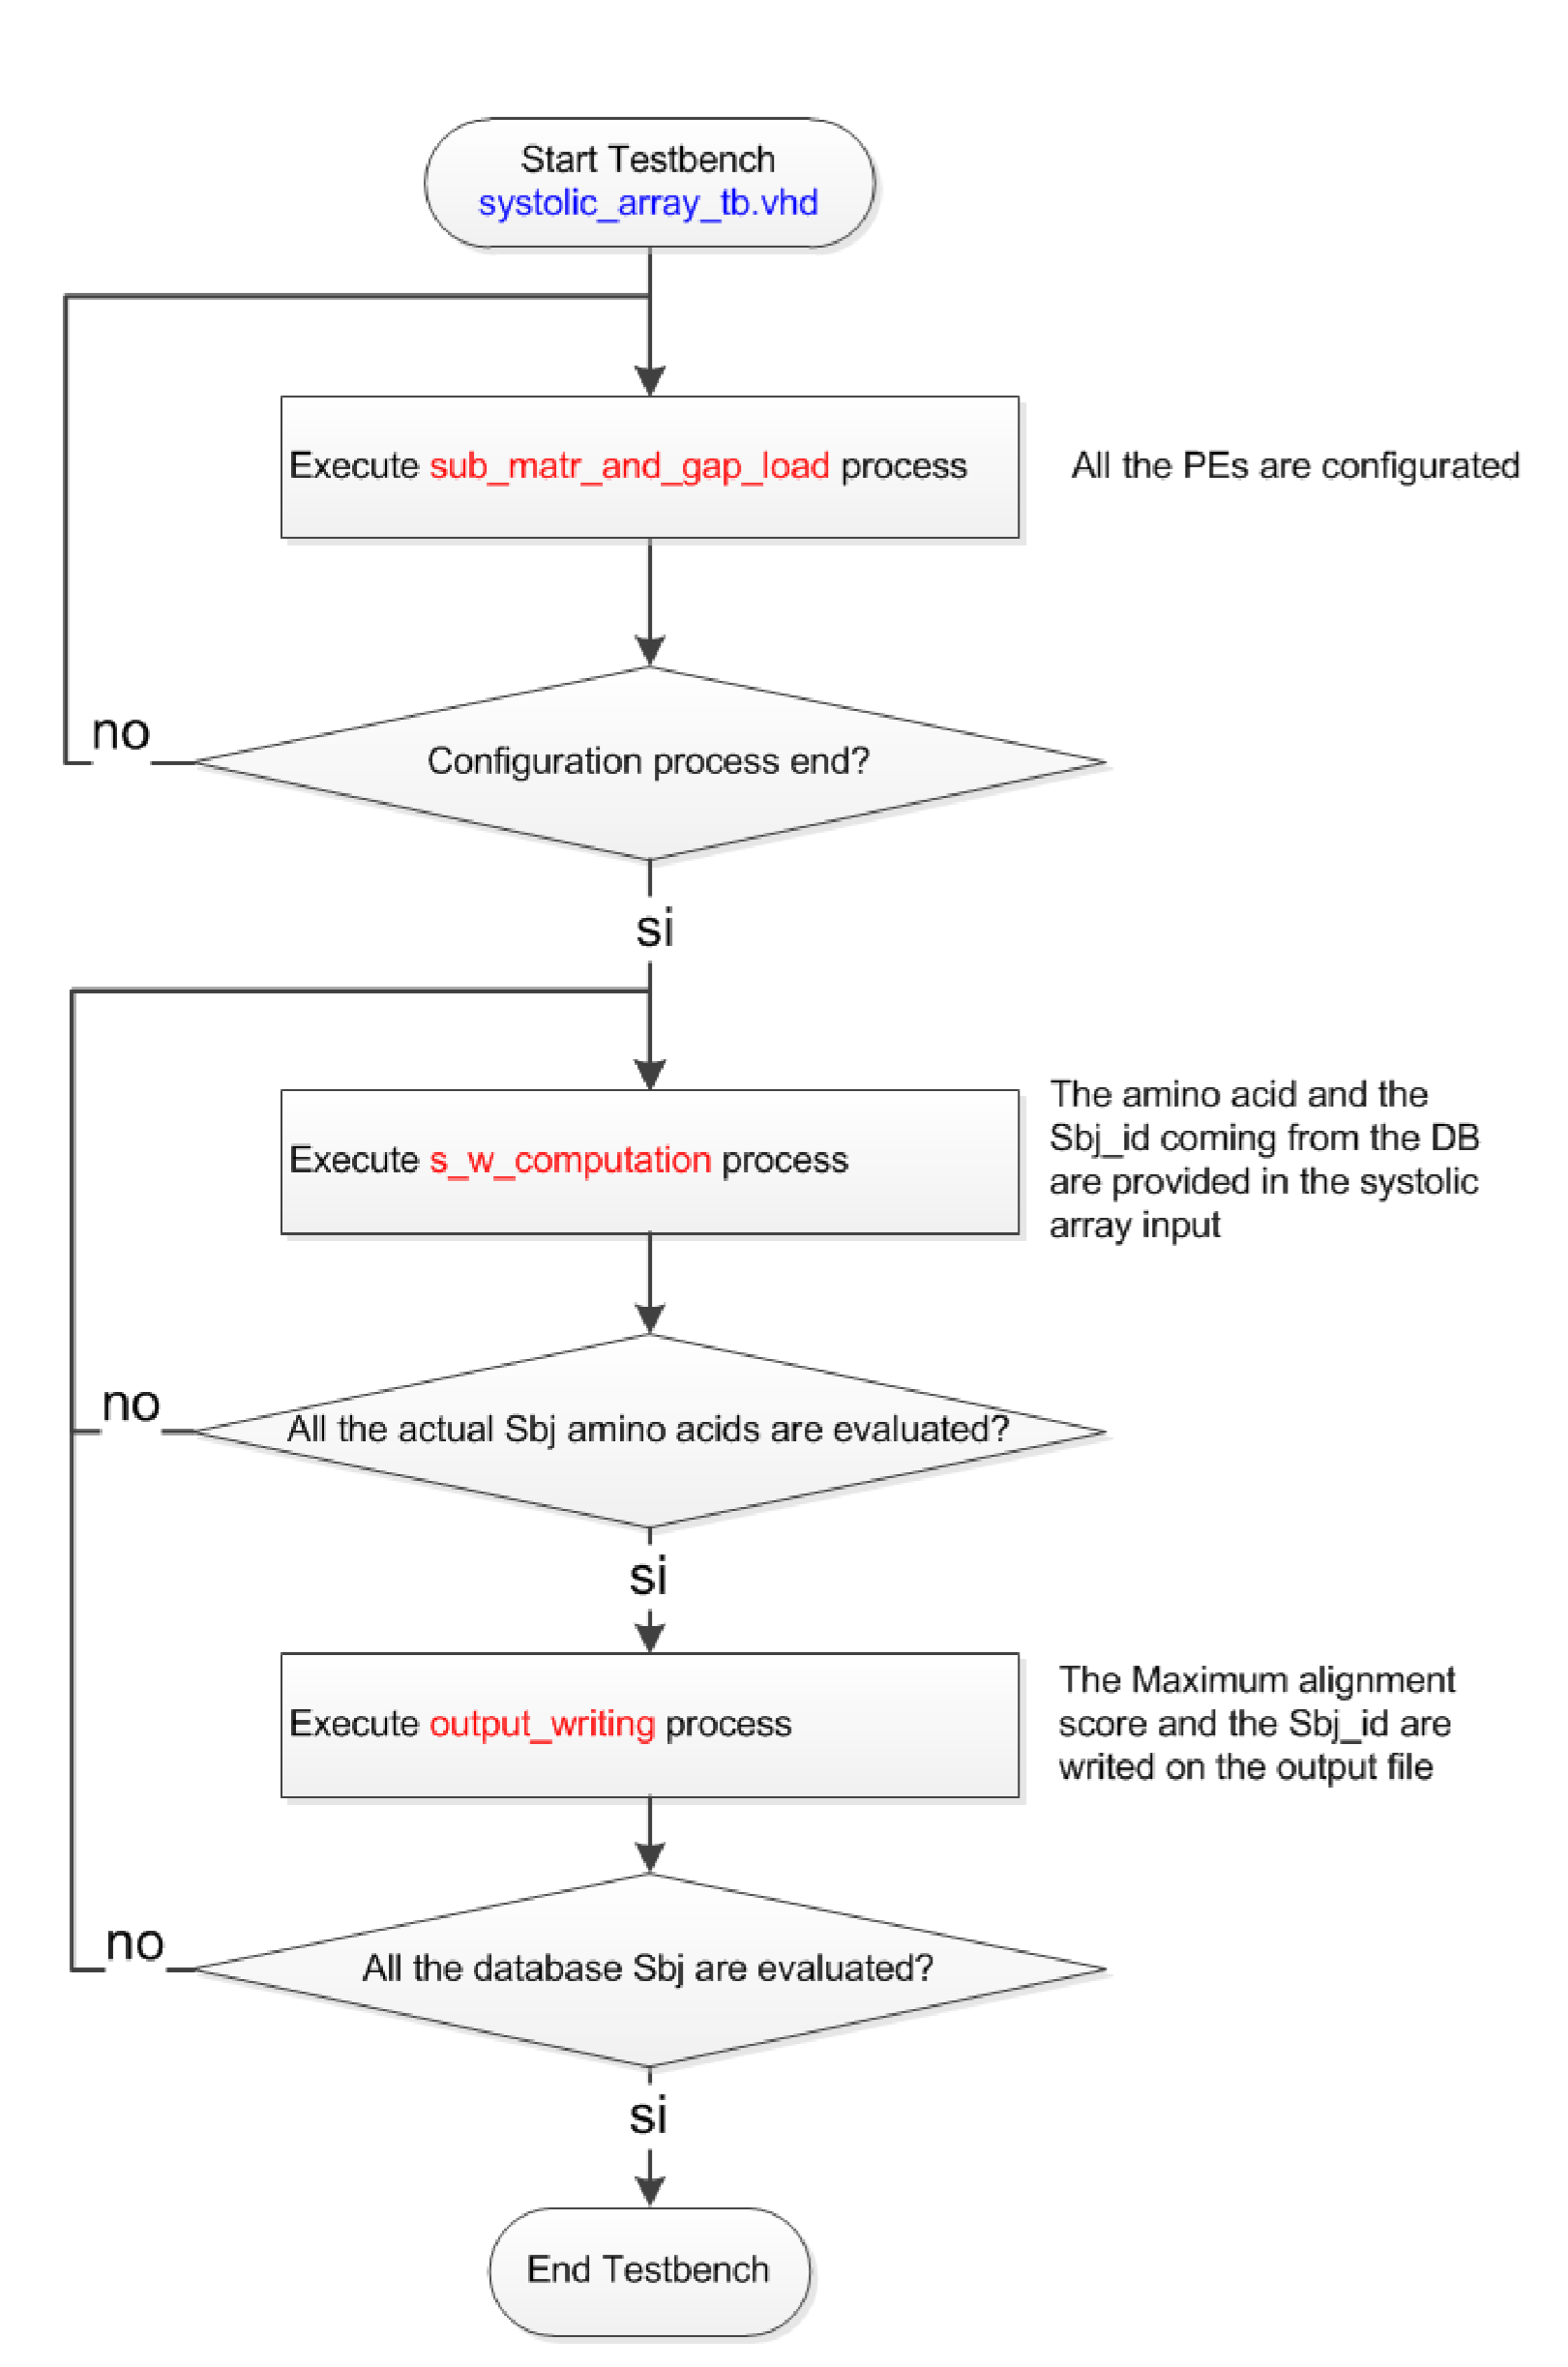
\includegraphics[width=0.7\textwidth]{imm/sw/tb_flow.png} 	\caption{Main flow chart of \textit{systolic\_array\_tb.vhd} testbench. In blue the testbench name, in red the processes name} 
	\label{tb_sw_flow}
\end{figure}

\clearpage
\newpage

\subsection{Phase 1-sub\_matr\_and\_gap\_load }
\begin{figure}[h!]
	\centering
	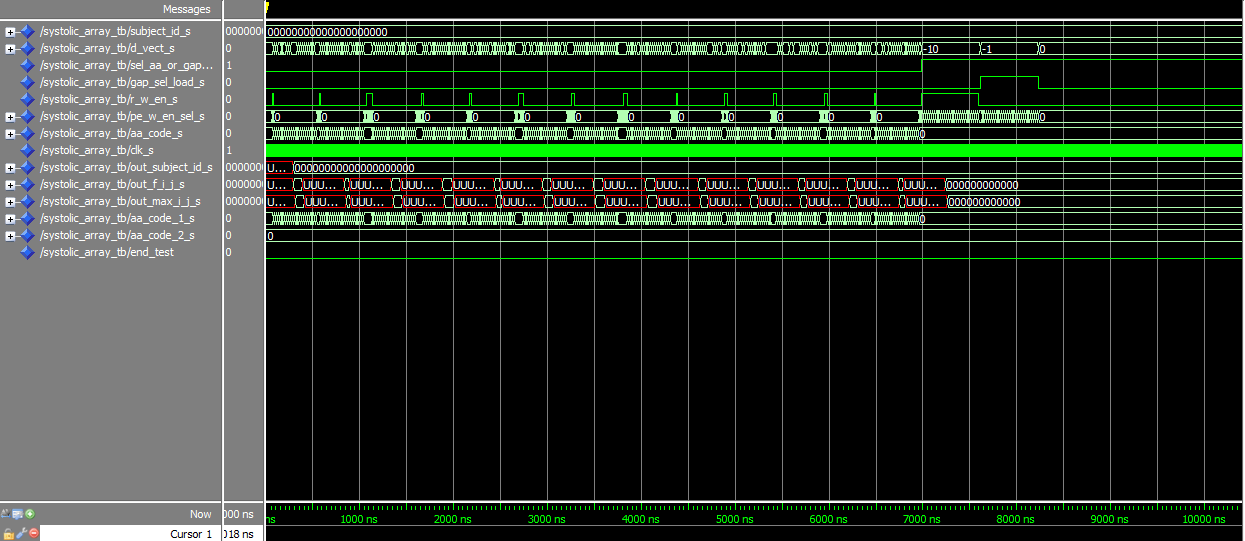
\includegraphics[width=\textwidth]{imm/sw/configuration_phase.png} 	\caption{Phase 1 of the testbench} 
	\label{tb_sw_1}
\end{figure}
In this phase we start to configure all the processing elements.\\
We need a file where are stored all the Qry AAs in the right format accepted by our testbench:\\
\textbf{out\_casual\_case\_config.txt} that is composed by:\\
\begin{itemize}
\item 23 rows that correspond to the used amino acids number. 
\item Each of these rows is associated to an amino acid (see fig. \ref{tabAA}). 
\item The first value of each row is the number of PE that must be loaded with the row associated to the amino acid. The following numbers identify the PE id number that must store the Substitutional matrix column. 
\item If the first value is 0 it means that the amino acid associated to this row is not present into the Qry.
\end{itemize}
\begin{figure}[h!]
	\centering
	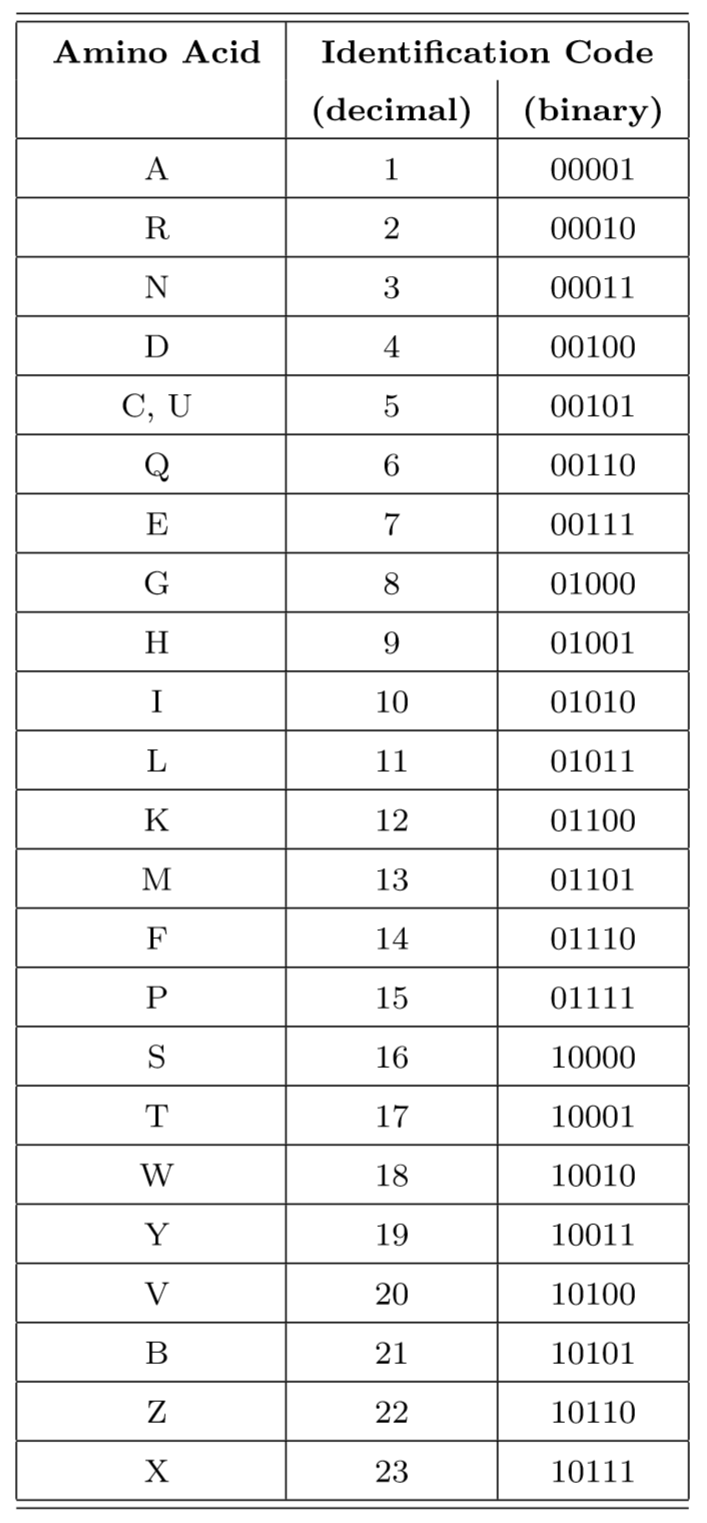
\includegraphics[height=0.95\textheight]{imm/sw/tabella.png} 	\caption{Amino acid encoding	} 
	\label{tabAA}
\end{figure}
\newpage
\RecustomVerbatimCommand{\VerbatimInput}{VerbatimInput}%
{fontsize=\footnotesize,
	%
	frame=lines,  % top and bottom rule only
	framesep=2em, % separation between frame and text
	rulecolor=\color{Gray},
	%
	label=\fbox{\color{Black}out\_casual\_case\_config.txt},
	labelposition=topline,
	%
	commandchars=\|\(\), % escape character and argument delimiters for
	% commands within the verbatim
	commentchar=*        % comment character
}
\VerbatimInput{file/out_casual_case_config.txt} \label{file_pes}

we can see that in the first rows it's written "1 \quad 17", that means that we need to store the similarity values (fig. \ref{blosum62}) of the first amino acid ('A') to the PE whose id is 17.
\begin{figure}[h!]
	\centering
	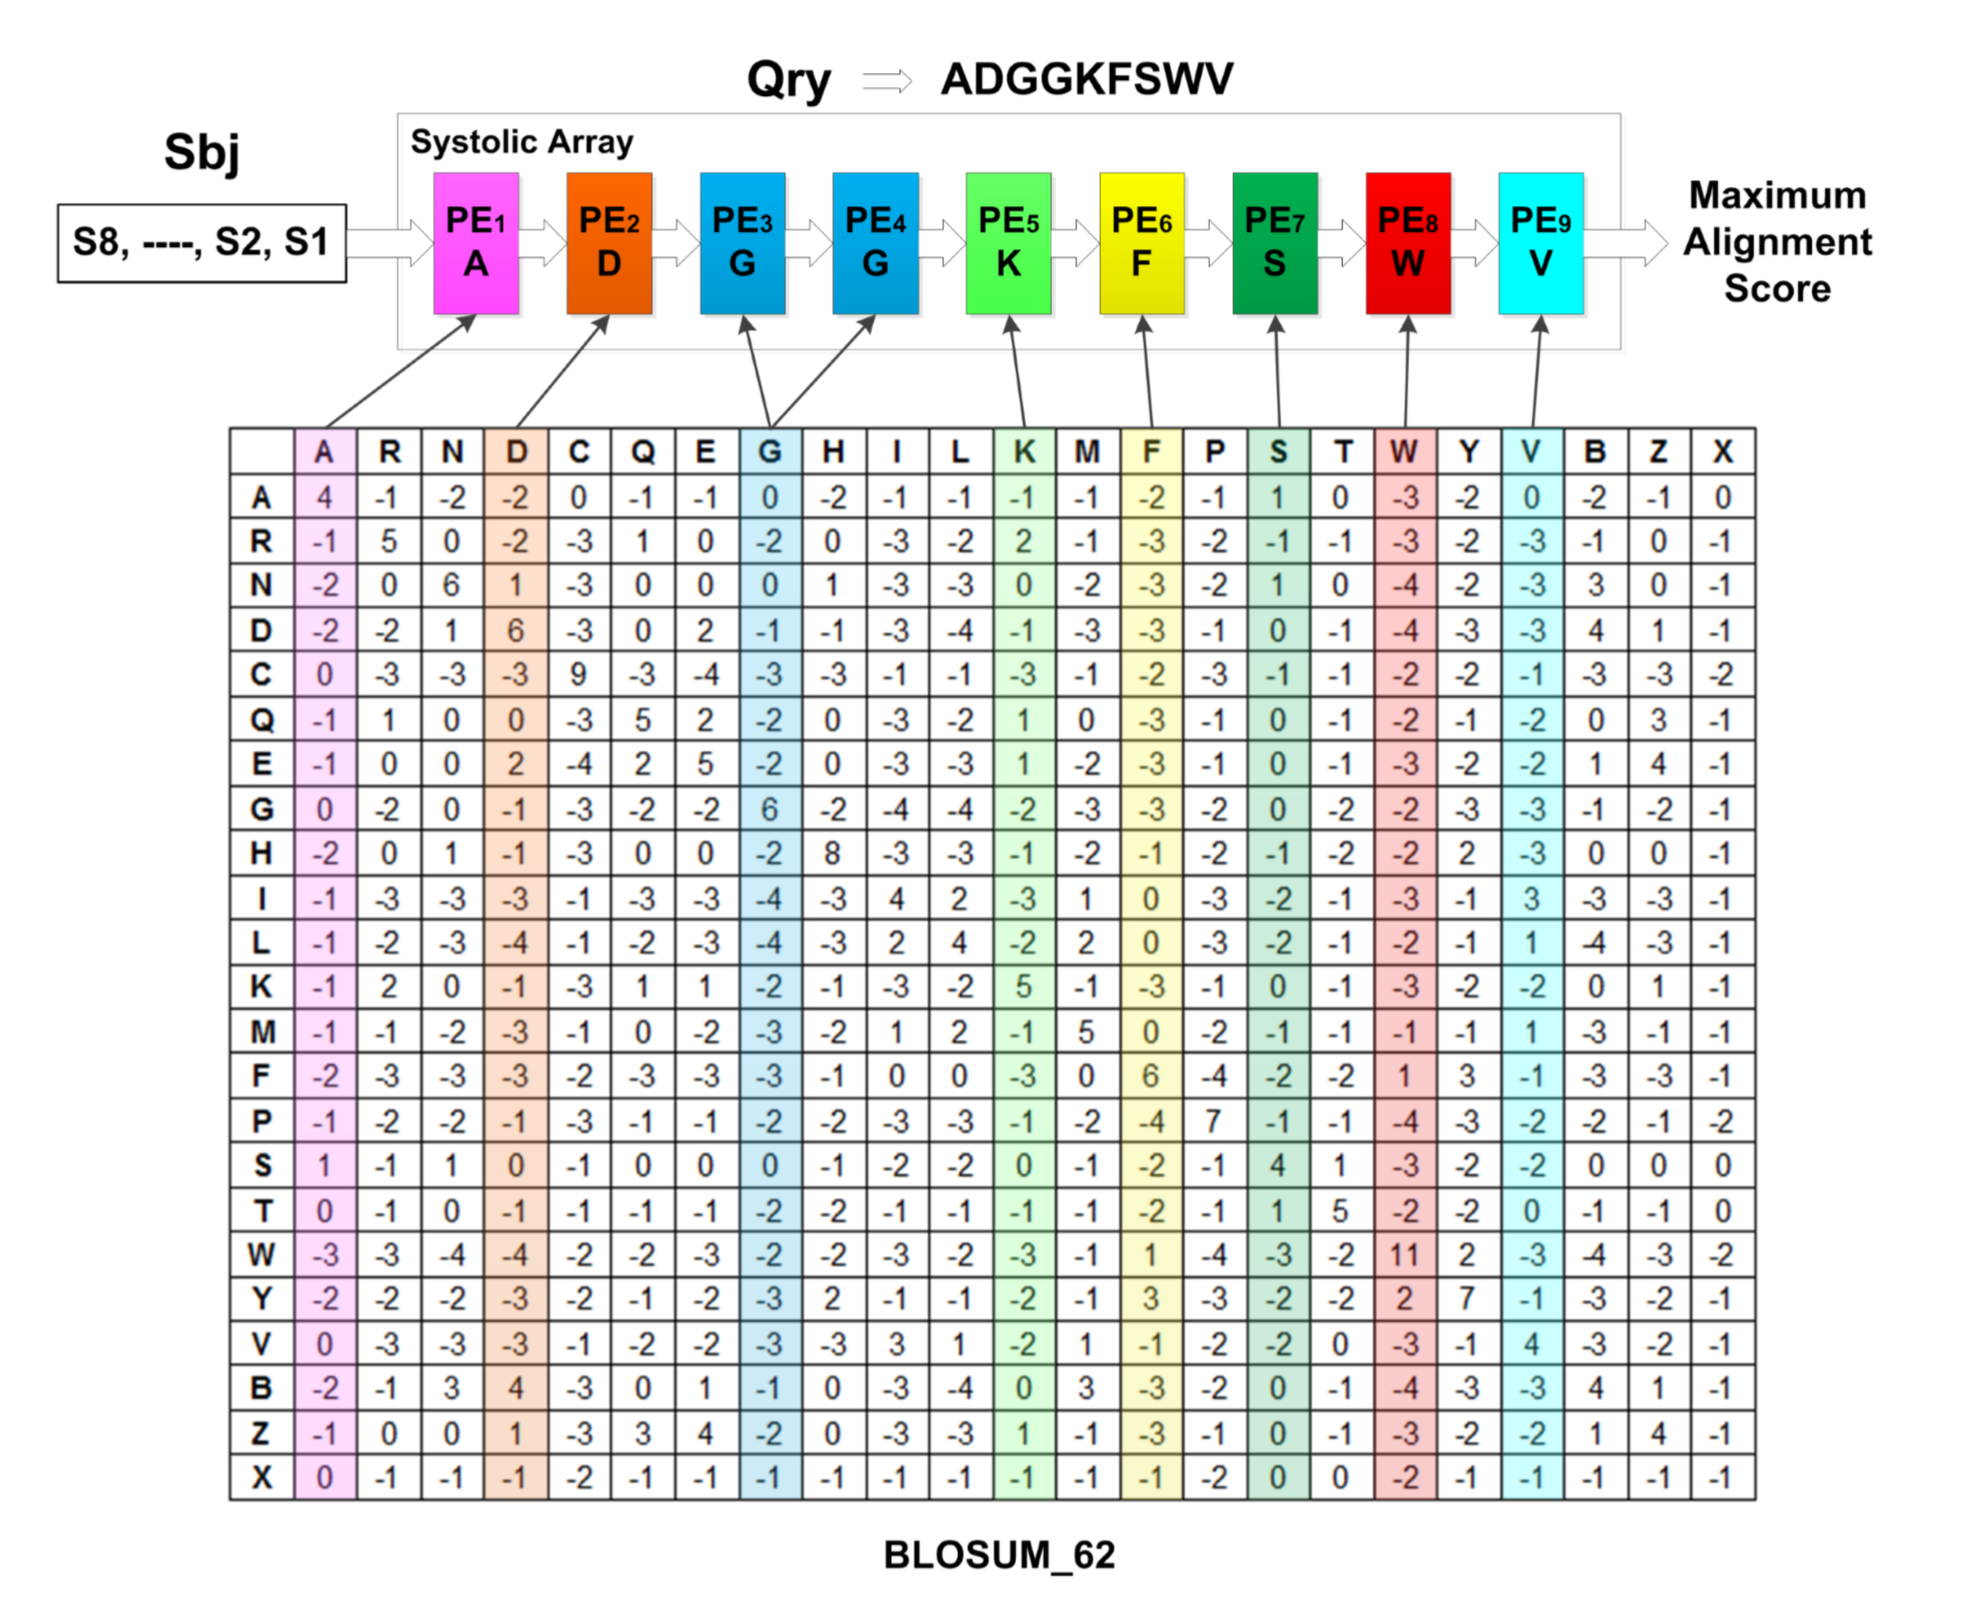
\includegraphics[width=\textwidth]{imm/sw/tb_sw1.png} 	\caption{S-W systolic array initialized with the Substitutional matrix columns: in each PE of the systolic array is stored the column that corresponds to the associated Qry amino acid.} 
	\label{tb_sw1}
\end{figure}

In other words we need to store in the 17-PE the values of the first column (the pink one in fig. \ref{tb_sw1}), as we can see also in the simulation (fig. \ref{tb_load_17})\clearpage
\begin{figure}[h!]
	\centering
	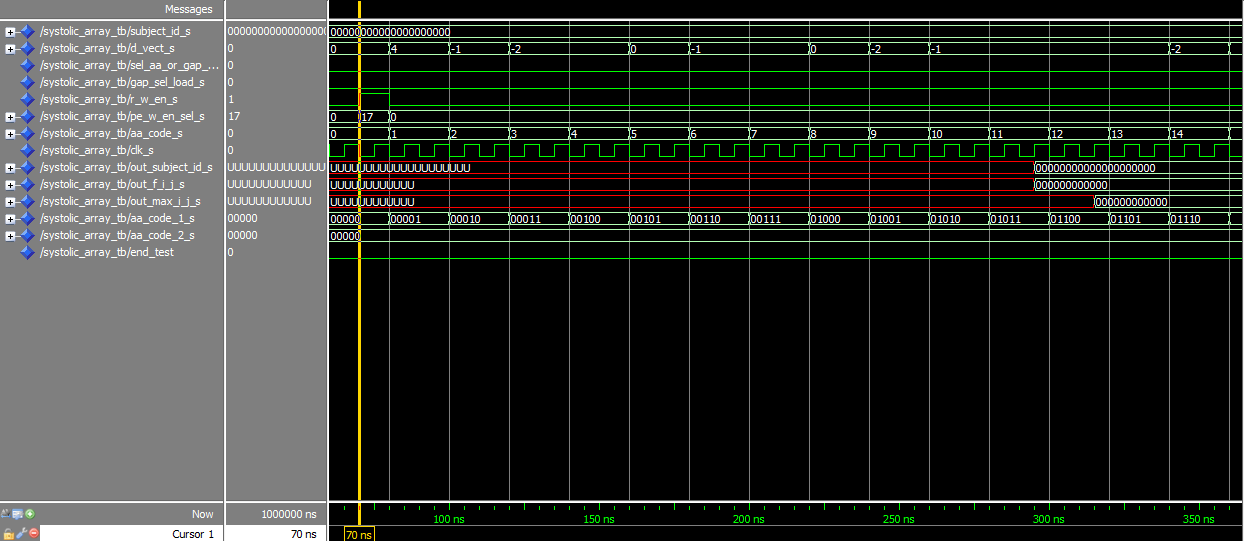
\includegraphics[width=\textwidth]{imm/sw/load_pe17_AA1.png}
	 	\caption{Loading into the 17-PE the Substitutional matrix column associated to the amino acid 'A'} 
	\label{tb_load_17}
\end{figure}

In the simulation we select the 17-PE ('\textit{r\_w\_en\_sel\_s}'=1 and '\textit{pe\_w\_en\_sel\_s}'=17 @ 70 ns ) then we load the substitutional matrix column associated to the amino acid 'A' (the pink one in fig. \ref{tb_sw1}).\\
\begin{center}
	
\begin{tabular}{|l|c|c|c|c|c|c|c|c|}

	\hline
	\textit{d\_vect\_s} & 4 & -1 & -2 & -2& 0 & -1 & -1& $ \dots $\\
	\hline
	\textit{aa\_code\_s} & 1& 2& 3 &4 &5& 6& 7 & $ \dots $\\
	\hline
	Amino Acid & A& R& N &D &C& Q& E & $ \dots $\\
	\hline
\end{tabular}\\ 
\end{center}
\begin{center}
	Loading for 17-PE
\end{center}\clearpage
The second row of the file \textit{out\_casual\_case\_config.txt} (as seen in section \ref{file_pes} has "1 \quad 19", so we do the same thing as before where we store the second column of the BLOSUM62 matrix (fig. \ref{tb_sw1}).\begin{figure}[h!]
	\centering
	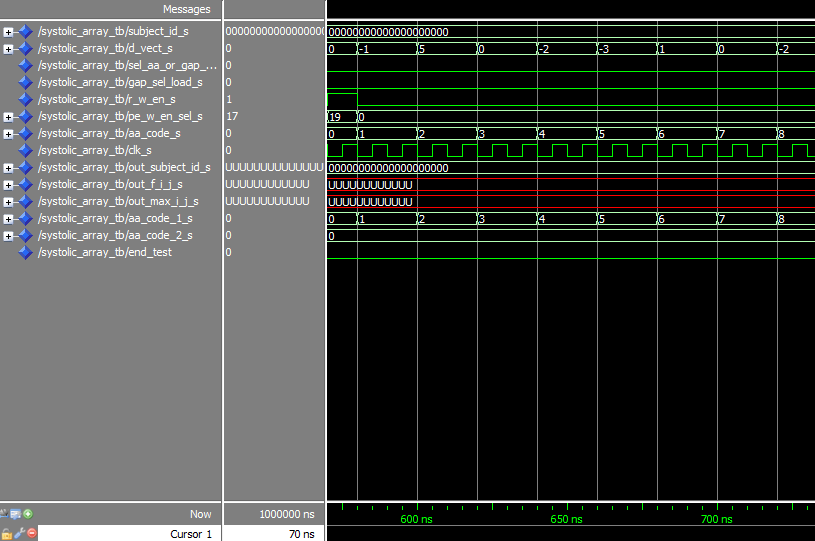
\includegraphics[width=\textwidth]{imm/sw/load_pe19.png}
	\caption{Loading into the 19-PE the Substitutional matrix column associated to the amino acid 'R'} 
	\label{tb_load_19}
\end{figure}
\begin{center}
	
\begin{tabular}{|l|c|c|c|c|c|c|c|c|}
	
	\hline
	\textit{d\_vect\_s} & -1 & 5 & 0 & -2& -3 & 1 & 0& $ \dots $\\
	\hline
	\textit{aa\_code\_s} & 1& 2& 3 &4 &5& 6& 7 & $ \dots $\\
	\hline
	Amino Acid & A& R& N &D &C& Q& E & $ \dots $\\
	\hline
\end{tabular}\\
\end{center}\begin{center}
Loading for 19-PE
\end{center}\clearpage
The third row has only the value '0', so no PE has to be configured for the third amino acid 'N'.\\
The fourth row has "5 \quad 5 \quad6 \quad12 \quad22 \quad27". Therefore we need to configure five PEs (i.e. 5, 6, 12, 22, 27) with the values associated to the Amino Acid 'D' (orange column in fig. \ref{tb_sw1}) as shown in fig. \ref{tb_sw_12}.
\begin{figure}[h!]
	\centering
	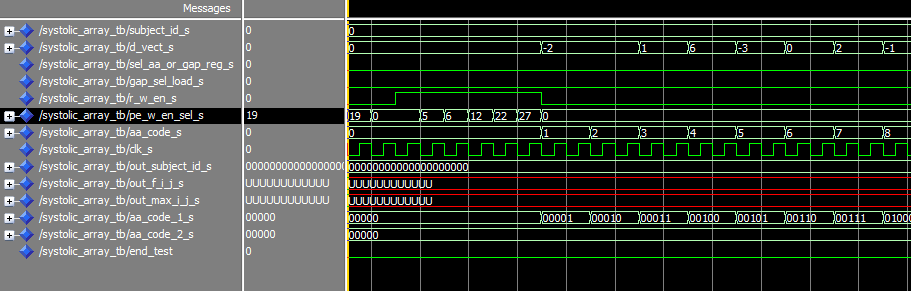
\includegraphics[width=\textwidth]{imm/sw/load_pe_5_6_12.png}
	\caption{Loading into the 5, 6, 12, 22, 27-PEs the Substitutional matrix column associated to the amino acid 'D'} 
	\label{tb_sw_12}
\end{figure}
\begin{center}
	
\begin{tabular}{|l|c|c|c|c|c|c|c|c|}
	\hline
	
	\hline
	\textit{d\_vect\_s} & -2 & -2 & 1& 6& -3 & 0 & 2& $ \dots $\\
	\hline
	\textit{aa\_code\_s} & 1& 2& 3 &4 &5& 6& 7 & $ \dots $\\
	\hline
	Amino Acid & A& R& N &D &C& Q& E & $ \dots $\\
	\hline
\end{tabular}\\

\end{center}
\begin{center}
	Loading for 5, 6, 12, 22, 27-PEs
\end{center}
We keep this process until we reach the last PE to be configured, which is the number 8 (row 20).\\At the end of this configuration (fig. \ref{tb_sw_pe8}), we need to store the two gap values (written in the file \textit{gap\_open\_ext.txt}) to all the PEs, the first value is the Open gap (fig. \ref{tb_open_gap_10}) while the second one is the Extension gap (fig. \ref{tb_ext_gap}).


The signal \textit{gap\_sel\_load} is high only when storing the extension gap, while \textit{sel\_aa\_or\_gap\_reg} is at '1' only when storing both the penalties (open and extension)
\begin{figure}[h!]
	\centering
	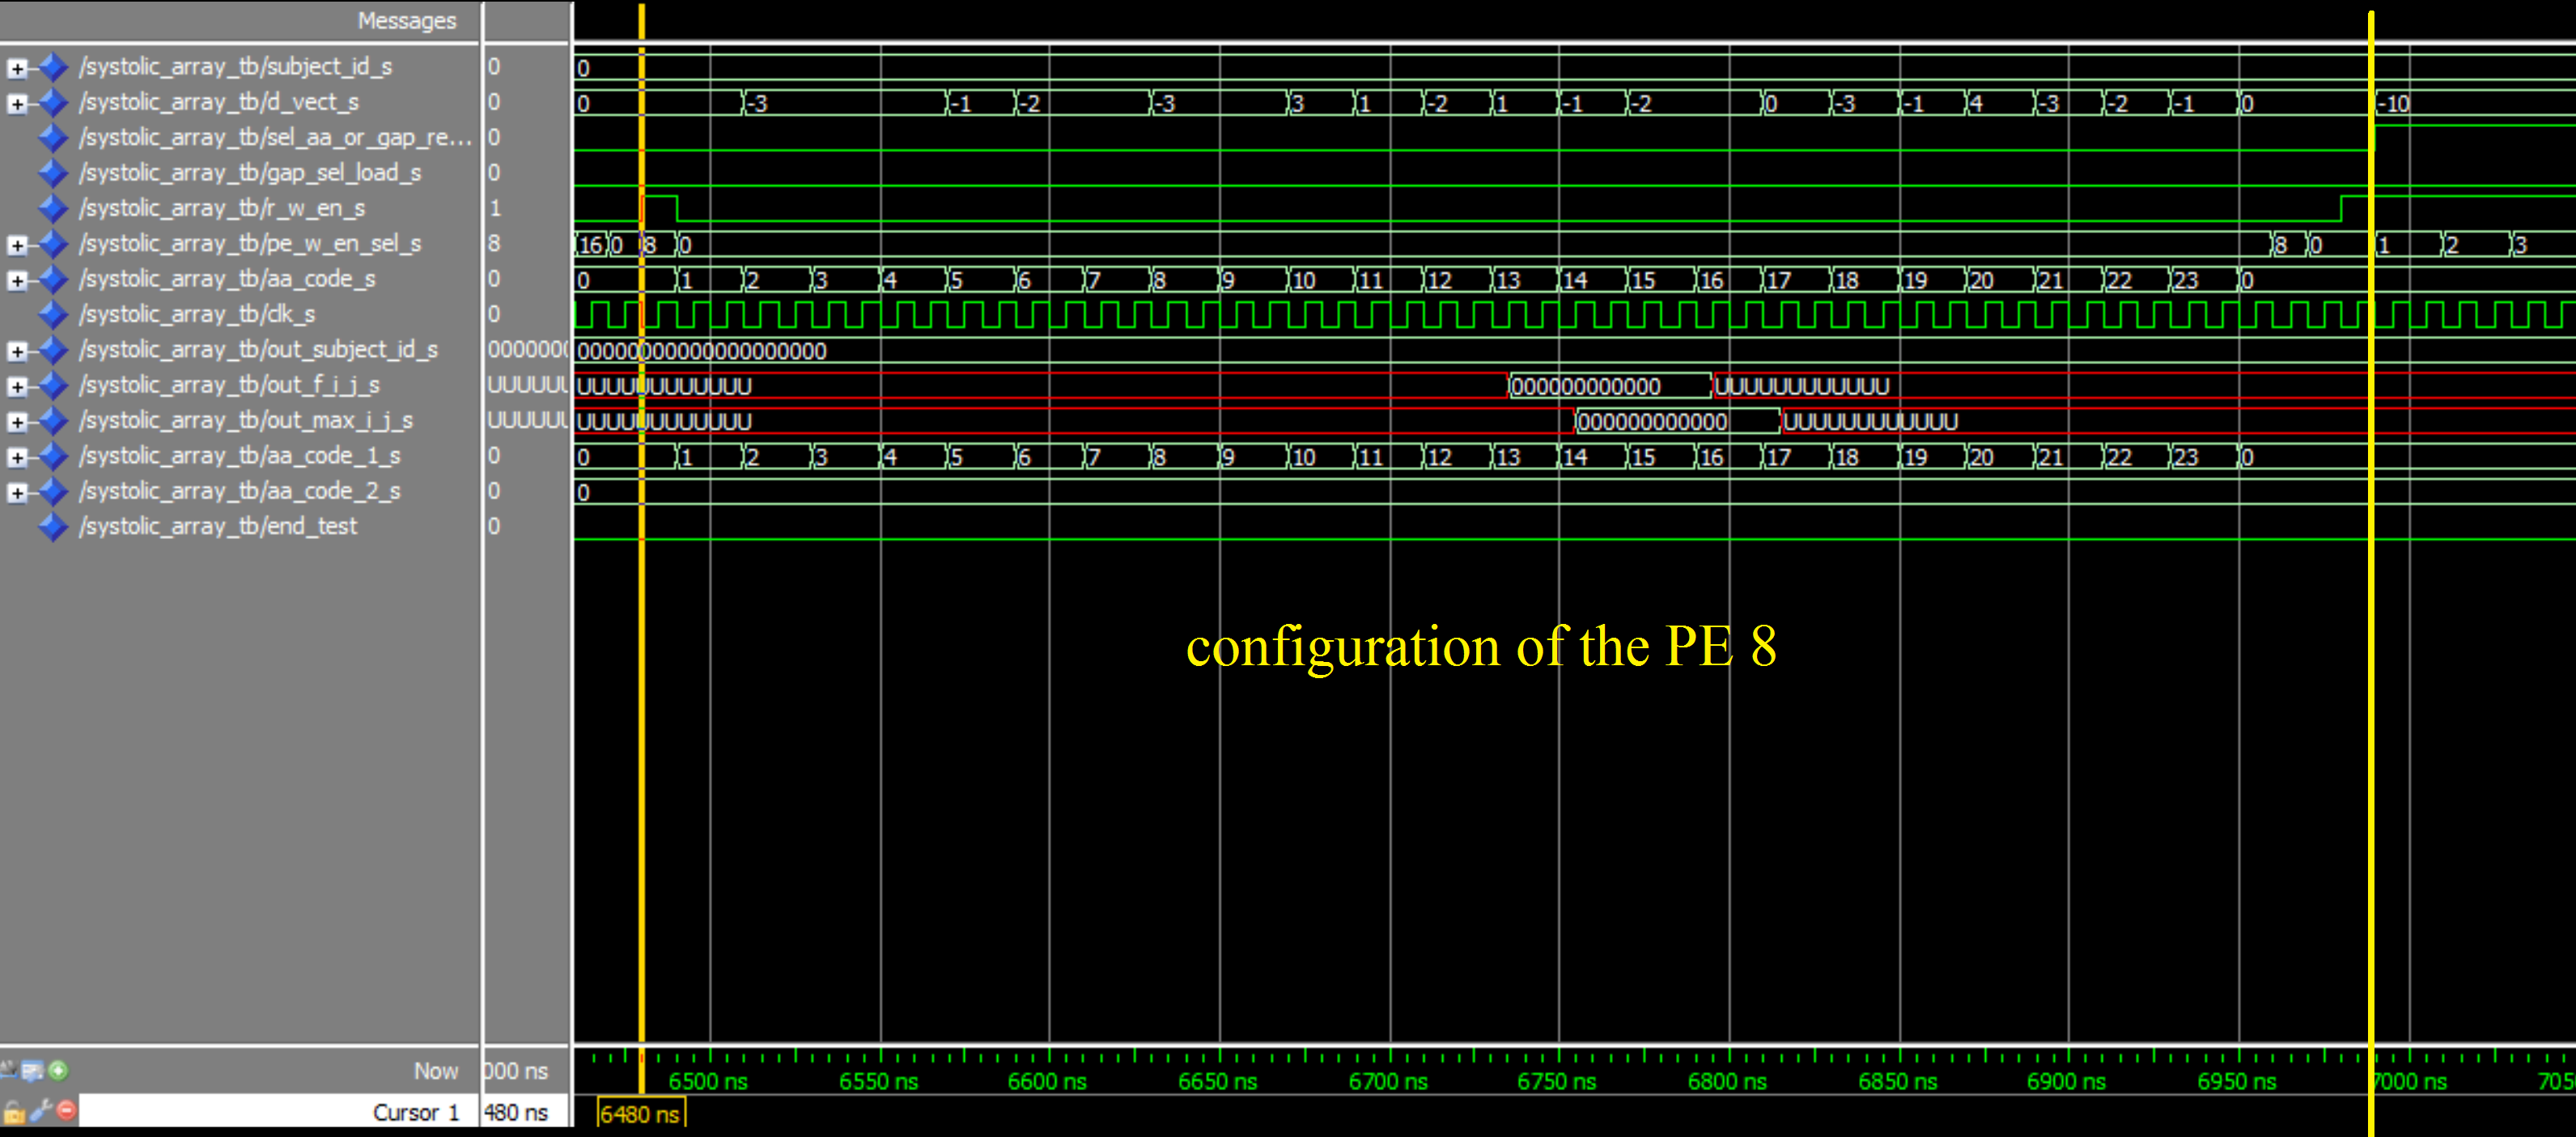
\includegraphics[width=\textwidth]{imm/sw/load_pe_8.png}
	\caption{Loading into the 8-PEs the Substitutional matrix column associated to the amino acid 'V'. On the right side, we see that we start to load the open gap penalty.} 
	\label{tb_sw_pe8}
\end{figure}
\begin{figure}[h!]
	\centering
	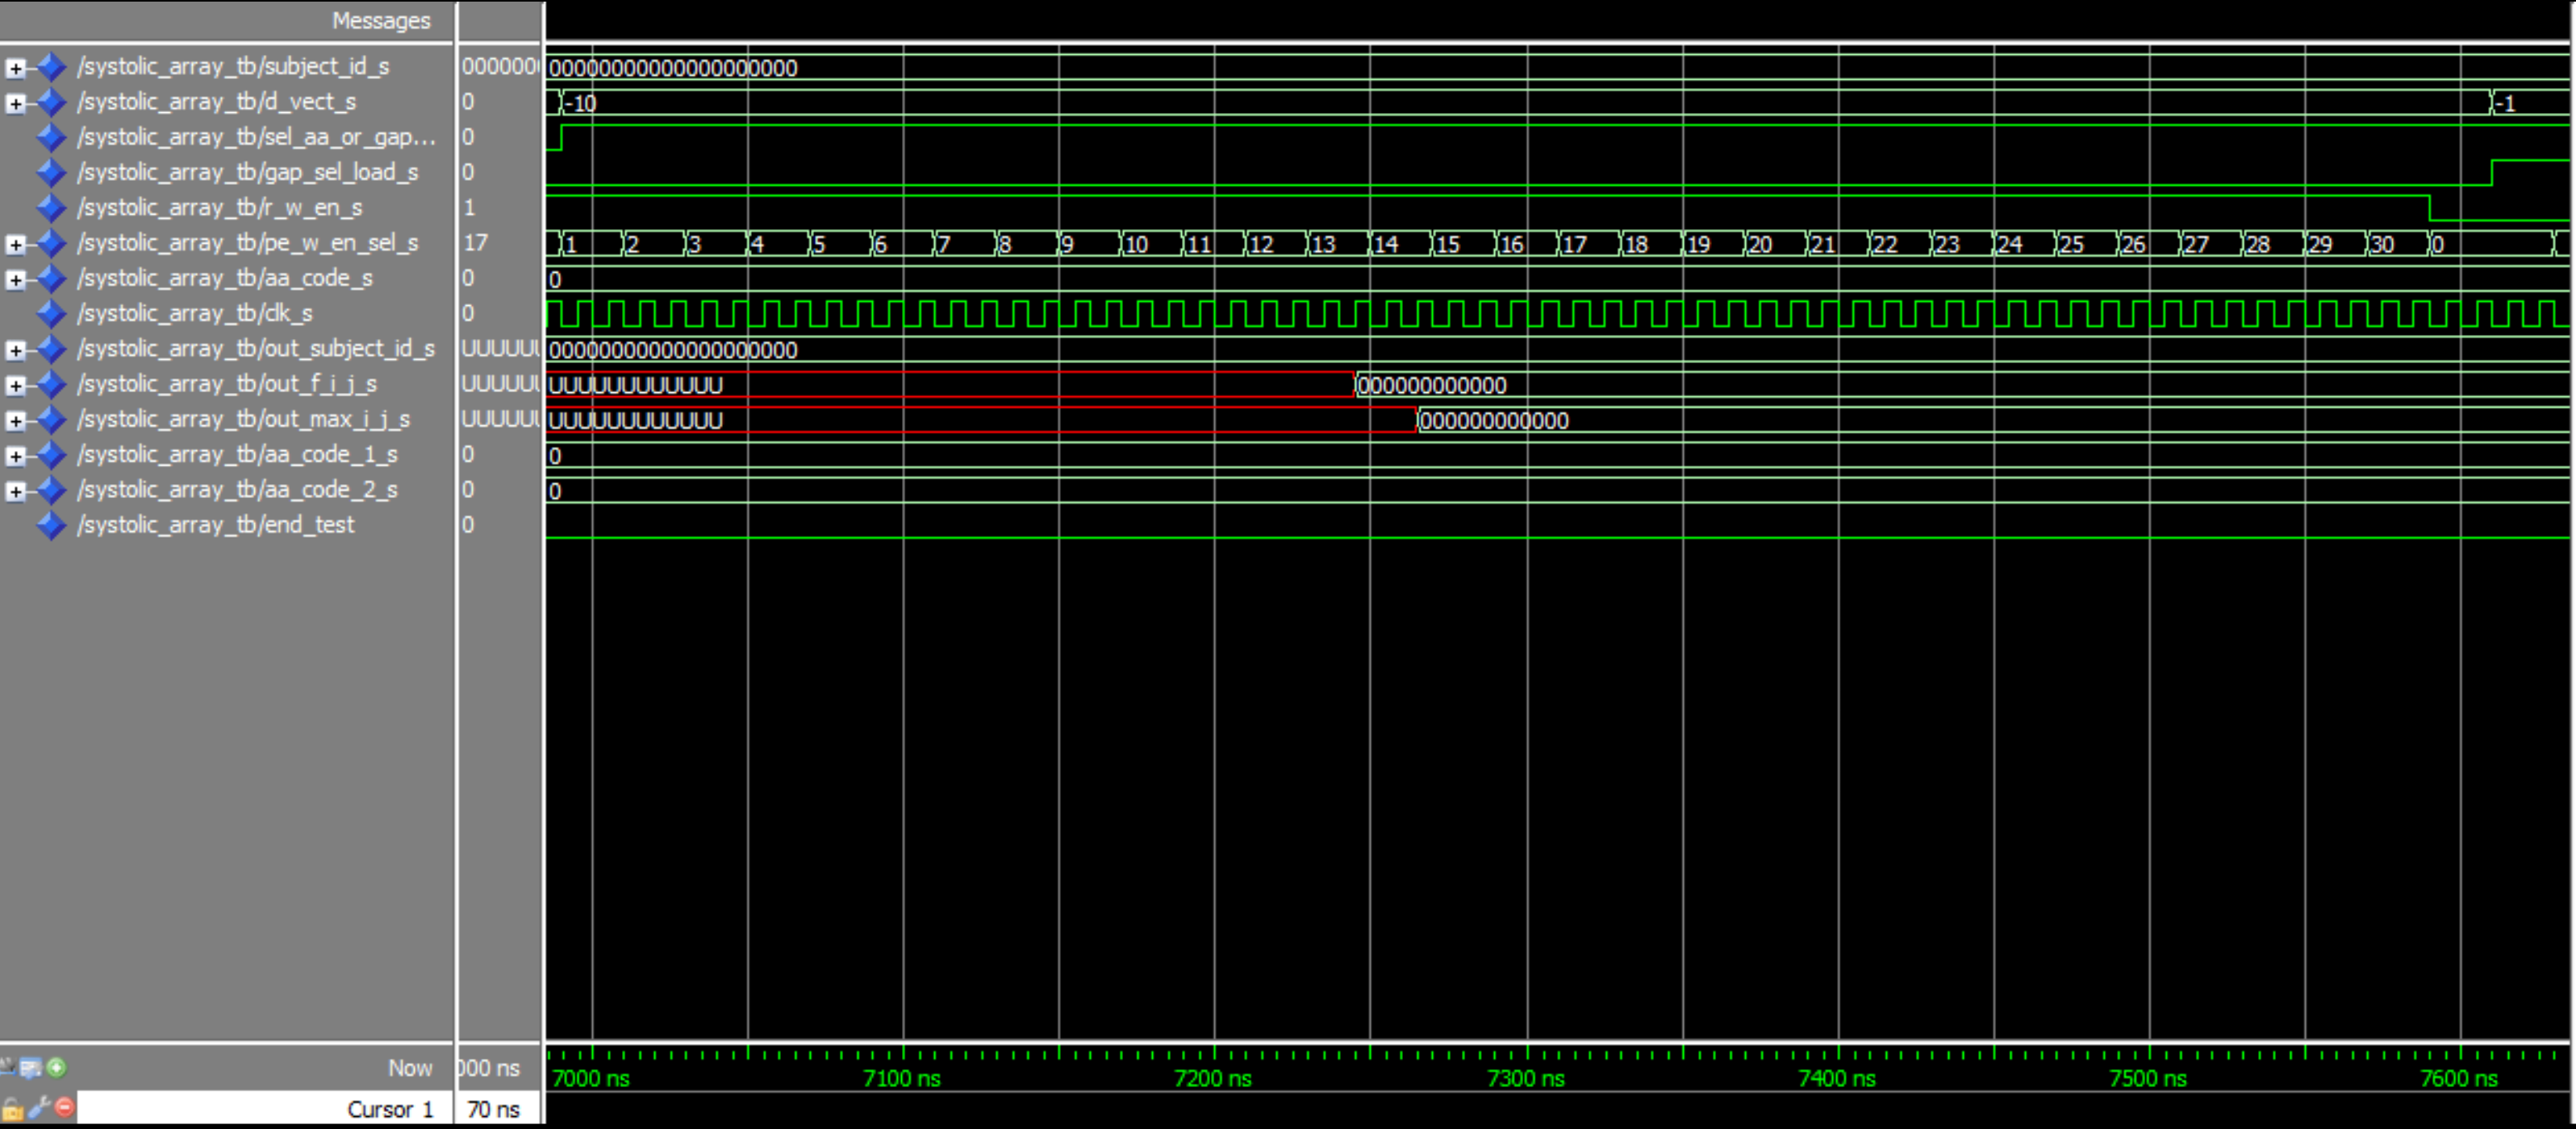
\includegraphics[width=\textwidth]{imm/sw/open_gap_10.png}
	\caption{Loading into all PEs the open gap penalty which value is -10} 
	\label{tb_open_gap_10}
\end{figure}
\begin{figure}[h!]
	\centering
	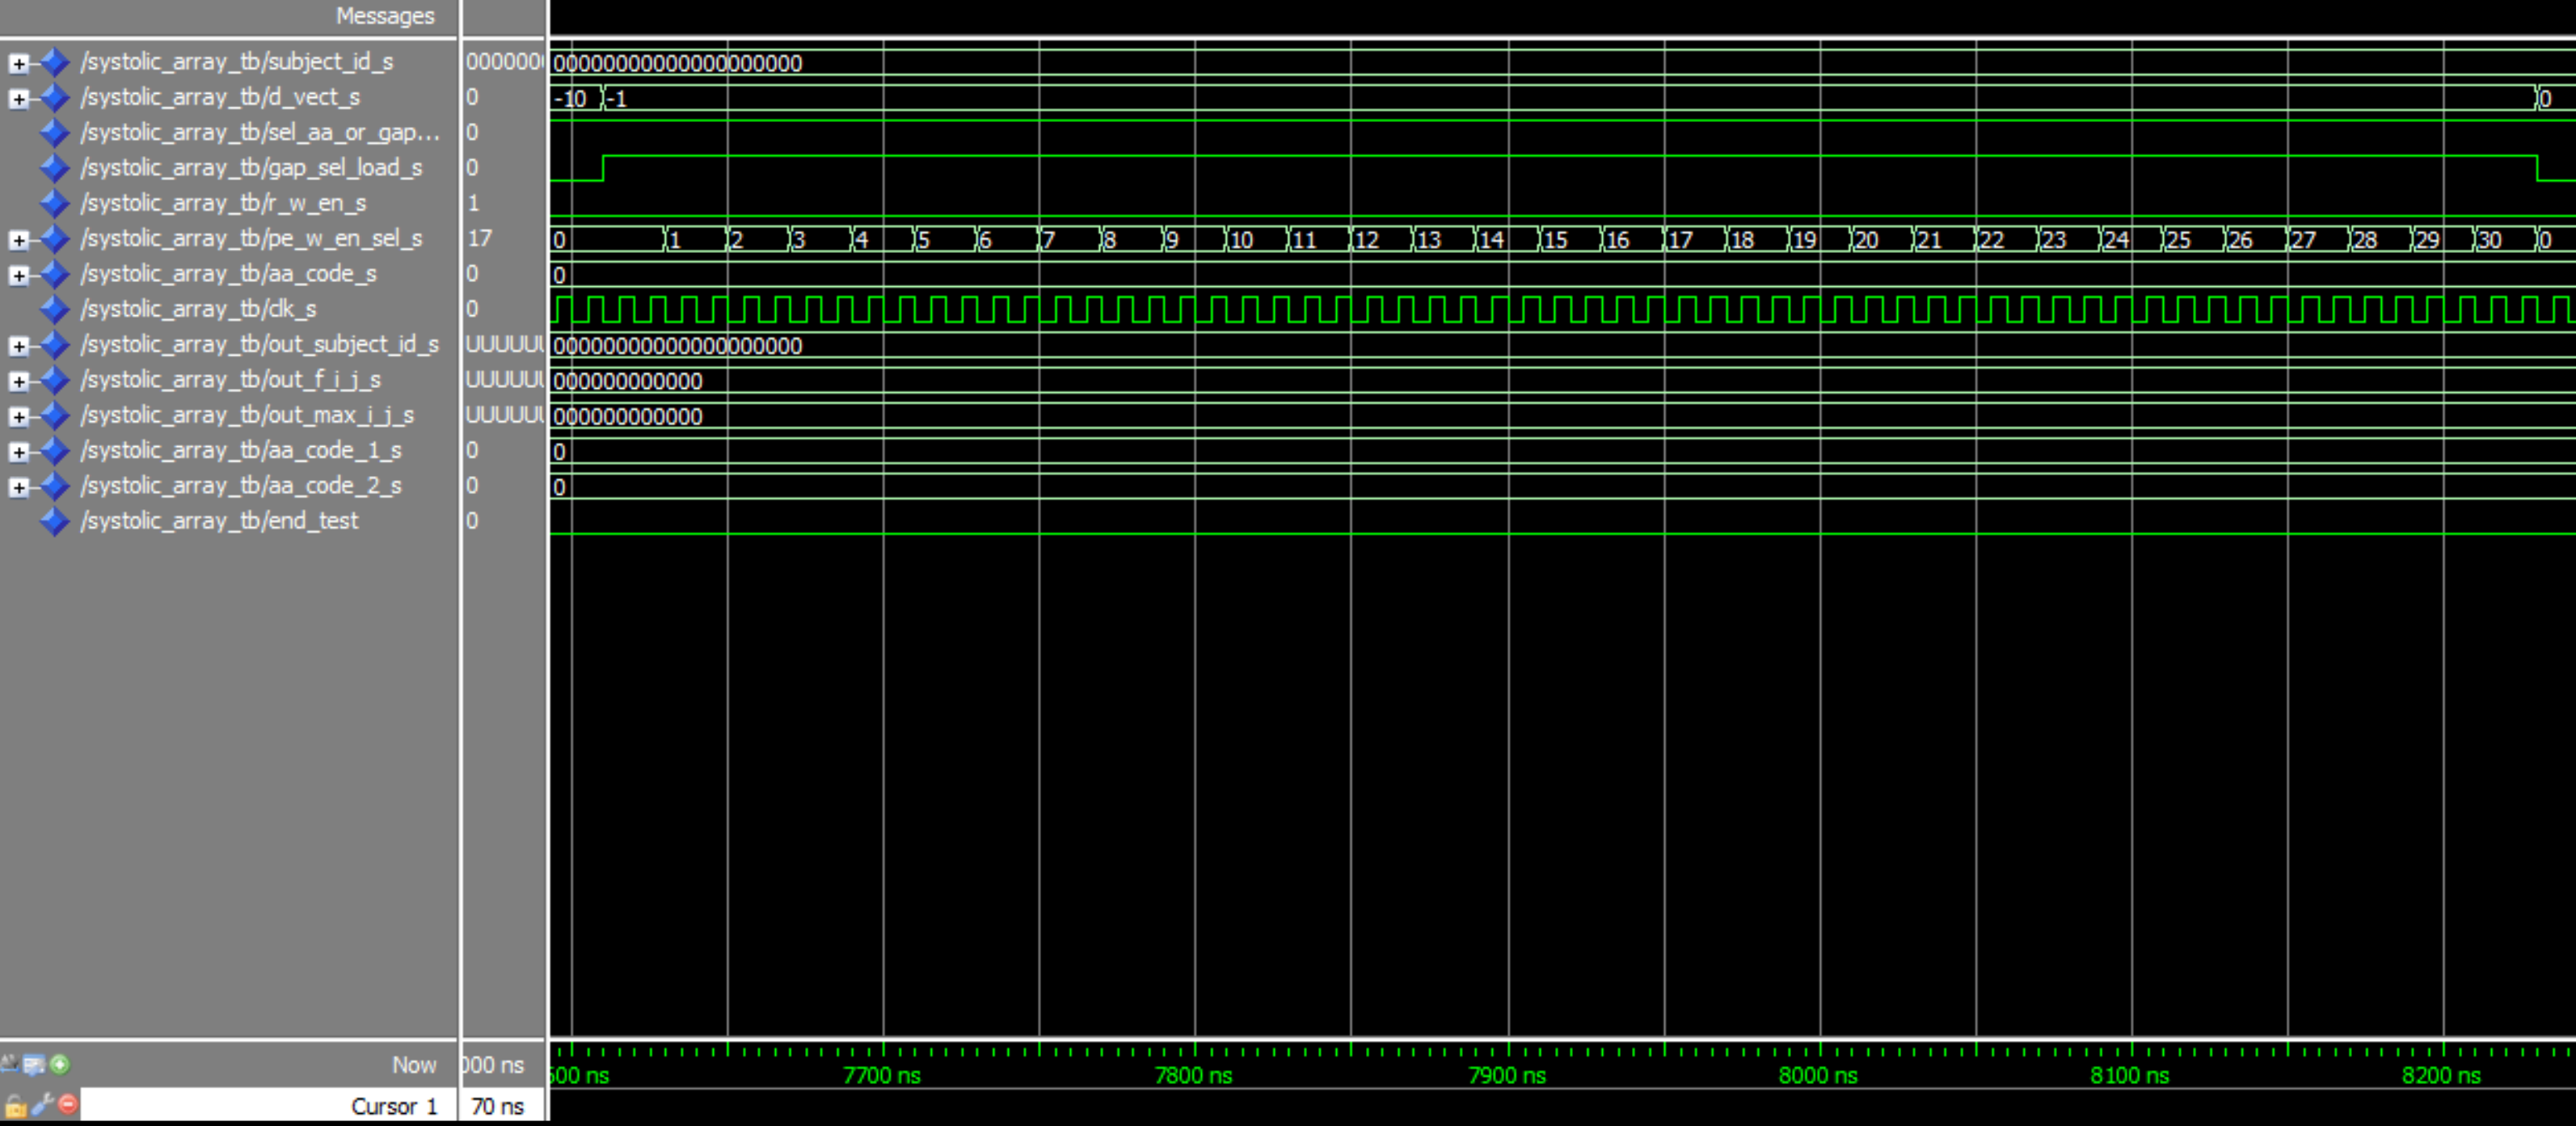
\includegraphics[width=\textwidth]{imm/sw/ext_gap.png}
	\caption{Loading into all PEs the extension gap penalty which value is -1} 
	\label{tb_ext_gap}
\end{figure}
\subsection{Phase 2- s\_w\_computation}
When the configuration phase ends, we can start the second process called \textit{s\_w\_computation}already explained in section \ref{simtest} and showed in fig. \ref{tb_sw}.
Here we scan the DataBase file \textit{DB\_num\_casual\_case\_2.txt} which is composed by:
 -In the first row of the file is written the number of sequences that compose this database.\\
 - In this file all the letters are converted in number using, for the conversion, a code that doesn't  take into account   the amino acids frequency (fig. \ref{tabAA}).
  The encoding code is written directly into the program.\\
   - The protein id number is the first value of the row (in this case 68). \\
   - The number of AAs that compose this protein is the second value in the same row.\\
    - All the other numbers are the encoded amino acids.
\begin{figure}[h!]
	\centering
	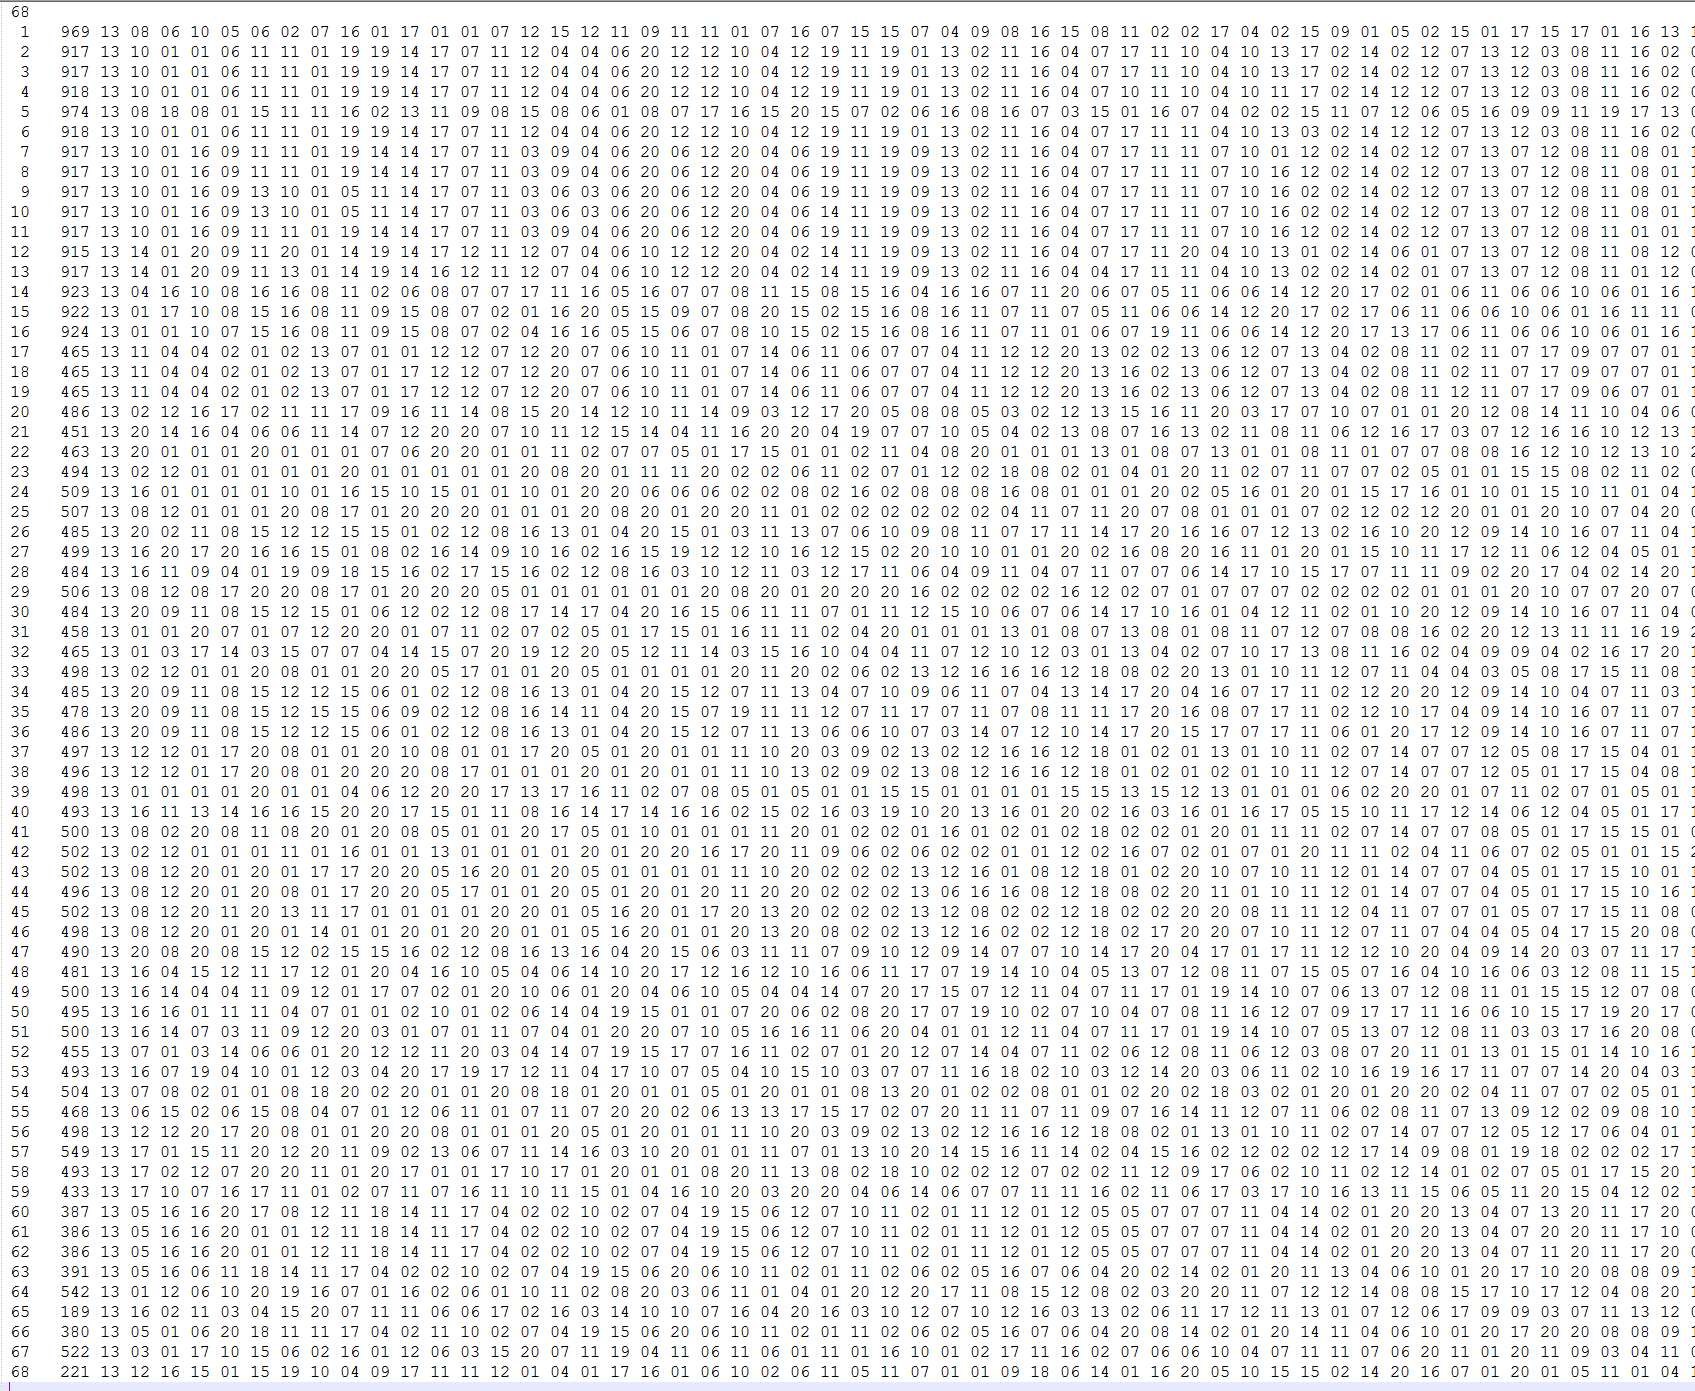
\includegraphics[width=\textwidth]{imm/sw/db.png}
	\caption{Section of the database file to be loaded in this testbench} 
	\label{db}
\end{figure}
\clearpage
\subsection{Phase 3- output\_writing}
In the \textit{subject\_id\_s} and \textit{out\_subject\_id\_s}, we can see the code for the selected protein, and in the \textit{aa\_code\_s} the proteins associated to such protein (the list of aminoacids is consistent with the database provided in the file \textit{DB\_num\_casual\_case.txt}).

\begin{figure}[h!]
	\centering
	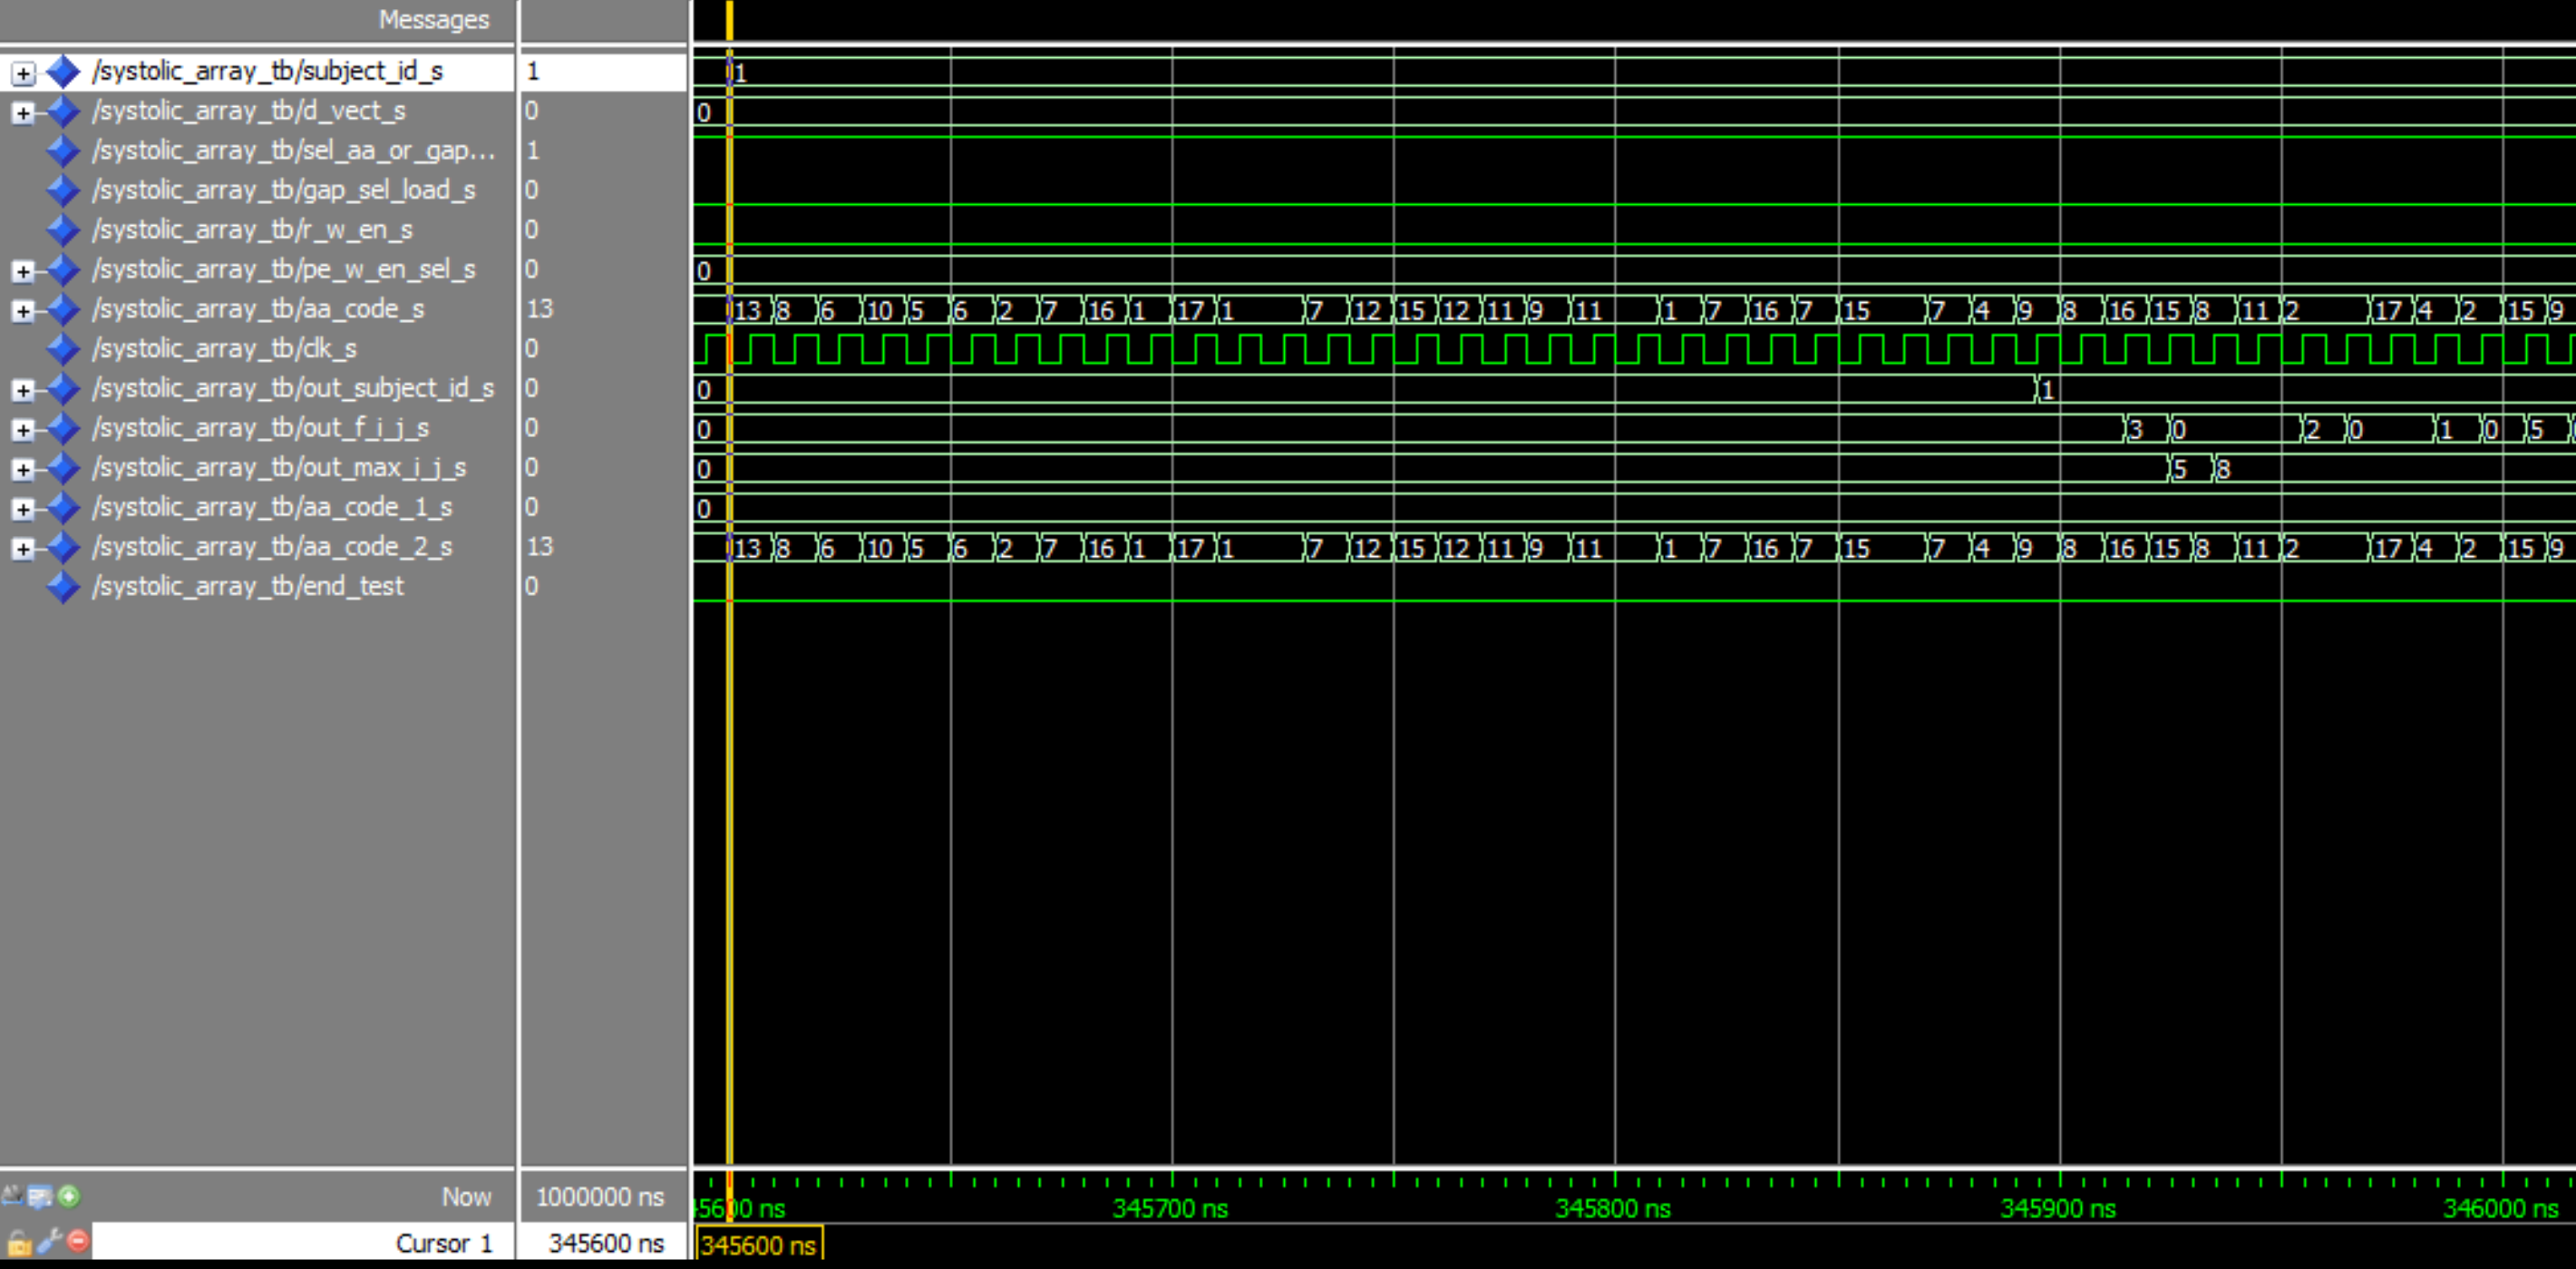
\includegraphics[width=\textwidth]{imm/sw/evaluating_output_1.png}
	\caption{scanning the list of aminoacid (\textit{aa\_code\_s}) of the first protein while computing the Maximum Alignment Score } 
	\label{output_evaluation_1}
\end{figure}

The\textit{ out\_f\_i\_j\_s} contains the Score matrix value calculated in the last PE (matrix cell F(i,j)) and the \textit{out\_max\_i\_j\_s} is the Maximum Alignment Score. Both these value are evaluated and shifted through the systolic array. As expected,  we can clearly see the Maximum Alignment Score increasing. In th fig. \ref{149} the value increases from an initial value of 5 to 149.
\begin{figure}[h!]
	\centering
	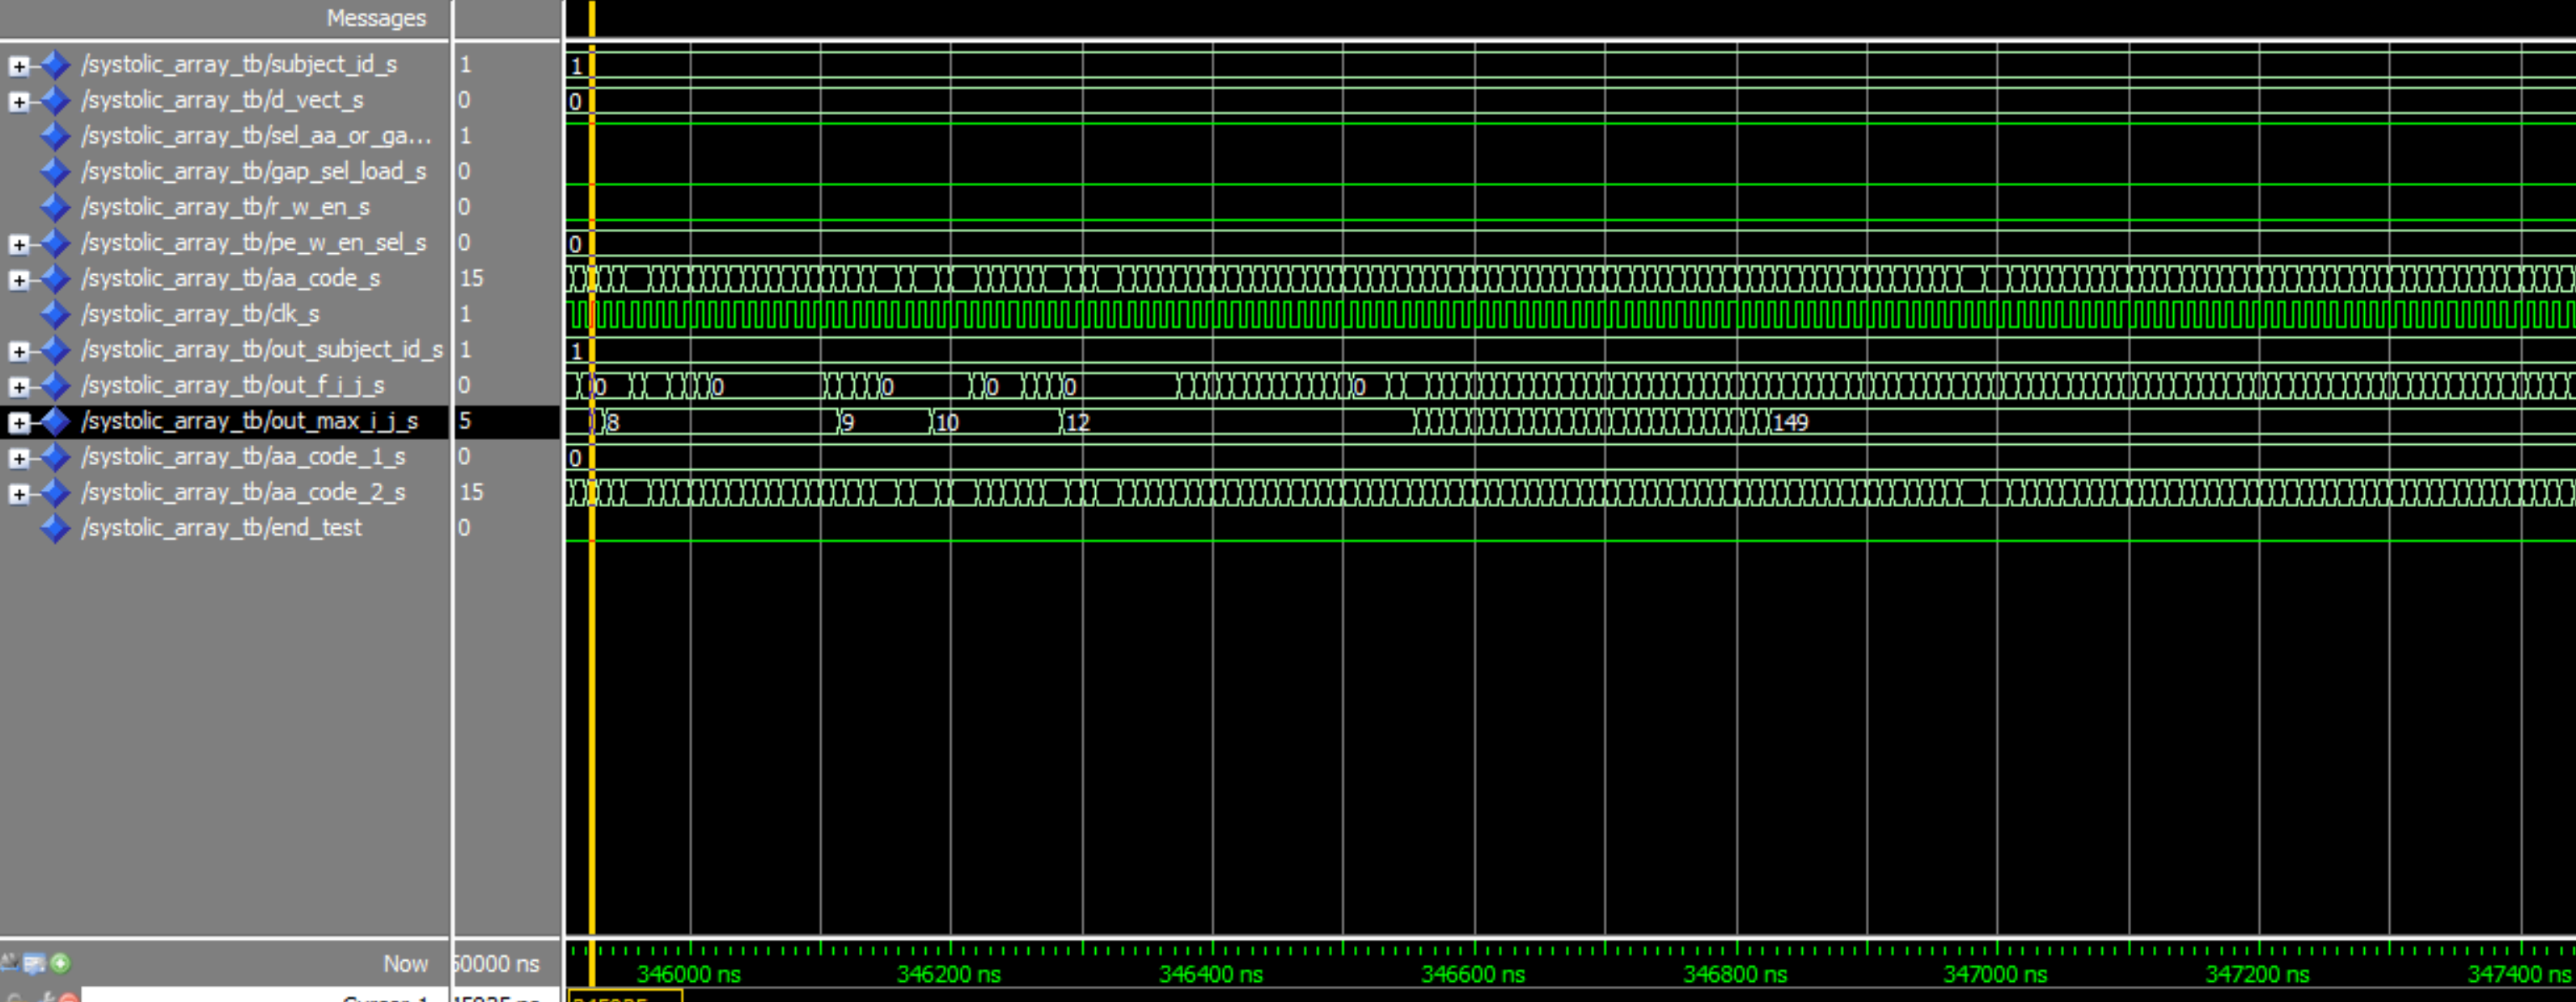
\includegraphics[width=\textwidth]{imm/sw/149.png}
	\caption{Computing the  Maximum Alignment Score (149) for the first protein } 
	\label{149}
\end{figure}
When all the process ends, we can write for each protein the Maximum Alignment Score evaluated in \textit{out\_id\_subj\_and\_max\_i\_j.txt} file

\begin{figure}[h!]
	\centering
	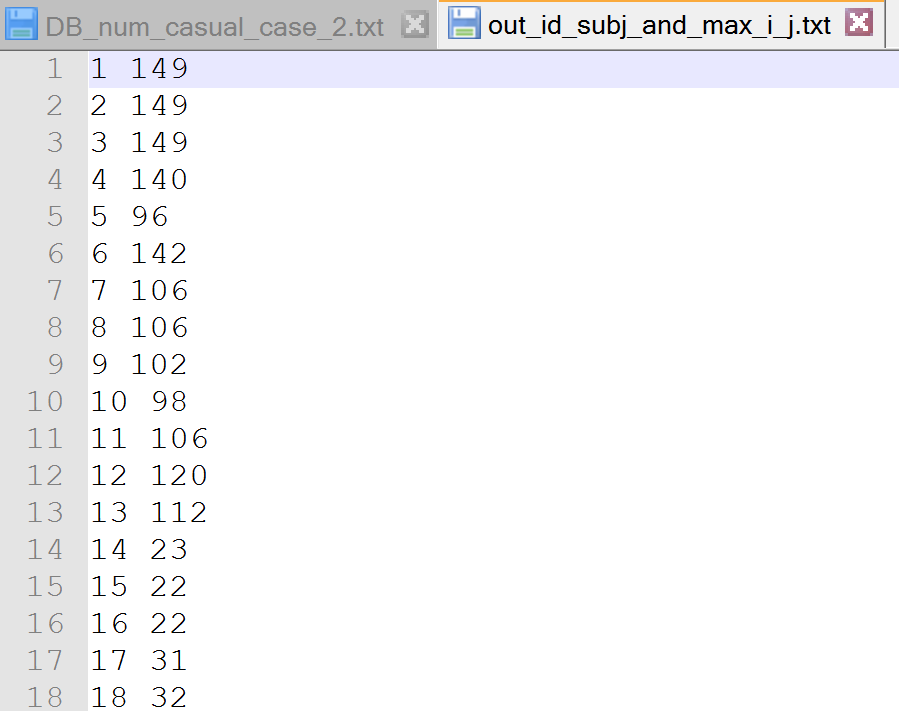
\includegraphics[width=0.5\textwidth]{imm/sw/out_149.png}
	\caption{In the first row of \textit{out\_id\_subj\_and\_max\_i\_j.txt} file we can see that the first protein has 149 as Maximum Alignment Score} 
	\label{out149}
\end{figure}
